\chapter{Analysis}

\red{CHAPTER STATUS: IN PROGRESS}


\section{Reconstruction and Tracking of SeaQuest Dimuons}

\subsection{Hit Reduction}

\subsection{Particle ID}

\subsection{Muon Momentum Reconstruction}

\subsection{Kalman Filter Track Fitting}

\subsection{Vertex Fitting}

\subsection{Monte Carlo Validation}

\section{Analysis Cuts}

The tracking software is concerned only with reconstructing possible tracks of relativistic charged particles through the SeaQuest spectrometer. It is, however, completely agnostic as to whether or not the charged particle was a muon that originated from a Drell-Yan interaction between the beam and the target. Though the tracker is agnostic as such, it should be noted that certain measures are in place in the design of the experiment that serve to increase the chances that a reconstructed track is a true DY muon track. Such examples are the choice of trigger matrix and the construction of an absorber wall before Station 4. Despite these measures, there are many cases in which we would wish to discard some signals, events, or whole spills in order to keep the data from becoming contaminated by anything but true $p-A$ Drell-Yan target dimuons.

As such, a set of cuts must be imposed to the tracked set of dimuon yields
\begin{itemize}
	\item Drell-Yan Selection Cuts: Exclude kinematic regions where the the signal is dominated by background
	\item Target Selection Cuts: Dimuons can be created in our beam dump. These cuts seek to remove the signals that likely originate from the dump.
	\item Trigger Selection Cuts: Many triggers were used to take data, and we only wish to analyze data triggered by a certain trigger configuration.
	\item Intensity Cuts: Data taken at unusually high intensities where components of the experiment can perform abnormally should be excluded.
	\item Quality Cuts: Most cuts fall under this umbrella. These include, but are not limited to: hardware settings, DAQ quirks, dimuon/track goodness-of-fits, etc.
\end{itemize}

In this section, these cuts are discussed in the order of tiers of data taking: Run, Spill, Event, Dimuon, Track. The intent with all of these cuts is to be as conservative as possible to ensure that all possible contamination is removed from the data despite the inevitable reduction in statistics.

\subsection{Data Selection}

The first cut on analyzable data is the choice of dataset to use. This document presents and discusses the EMC ratio results for SeaQuest roadsets \#57, \#62, and \#67. Each of these roadset settings were in place for the span of months and contain varying amounts of statistics. In total, many millions of tracks and dimuons of varying quality are found through the track reconstruction and vertex fitting procedure discussed in the previous section. Several cuts regarding quality of track/dimuon fit and experimental conditions are discussed below and applied to these datasets in order to isolate signal dimuons from the \emph{target}.

The names of the SeaQuest MySQL merged productions along with their date range, magnet polarity, respective statistics, and notes regarding roadset differences are presented in Table~\ref{tab:roadset-stats}.

\begin{table}
	\centering
	\caption{The experiment-specific data sources and their details.}
	\label{tab:roadset-stats}
	\begin{tabular}{c|rrr}
		Schema & Date Range & \# Dimuons & Roadset Notes\\	
		\hline
		merged\_roadset57\_R005\_V001 & dummy & dummy & dummydummydummy \\
		merged\_roadset62\_R005\_V001 & dummy & dummy & dummydummydummy \\
		merged\_roadset67\_R005\_V001 & dummy & dummy & dummydummydummy
	\end{tabular}
\end{table}

\subsection{Run Level Cuts}

It is an outspoken goal of the SeaQuest collaboration to absolutely keep as much data as possible. This means, in general, that the largest chunk of data that we want to allow to be thrown away is on a spill-level. That withstanding, there are a certain set of factors that could lead an entire run's ($\sim$\unit[1]{hr}'s) worth of data to be excluded.

One factor is the amperage settings of the focusing and spectrometer magnets. If these are not set nominally (\unit[2000]{A} and \unit[1600]{A}, respectively), the tracking will improperly reconstruct tracks, as it depends on a specific $p_T\text{-kick}$ value from each magnet in order to discern sensible tracks from the data. For this reason, if the averaged magnet currents are below 50\% of their nominal values, the run is excluded from analysis.

Another crucial characteristic for a run is if it contains Spill values. This can be attributable to a malfunction in the Beginning of Spill / End of Spill triggers or a malfunction in the Spill Counter function. Regardless of cause, without this spill label, it becomes impossible to relate data taken to any other critical values such as target position or beam intensity.

The rest of the run-level cuts can be summarized by the umbrella term of ``DAQ issues''. If the Slow Control failed to be recorded for any reason and there are zero Beam, Target, or Environment table values in a run, it is excluded. The same goes for the BeamDAQ and Scaler readouts. Perhaps most prevalent of the DAQ issues is the case of a run that failed upon starting. These resulted in empty \unit[32]{kB} files with no usable data.

Beyond these issues, there are also ranges of runs for which there was some larger issue at hand. The best example of this is the period of data taking during Roadset 62 where the automatic target control was malfunctioning. The shift crew controlled the target position manually, but the actual target that was in the path of the beam during the spill could not be verified. As such, these runs were excluded. There is very little indication from the data itself that would incriminate itself as being untrustworthy, and so these are specifically excluded by analyzers. In practice, the runs are removed from the data set via an excluded range of spillIDs.

\subsection{Spill Level Cuts}

\begin{table}
	\centering
	\ra{1.3}
	\setlength{\tabcolsep}{2em}
	\begin{tabular}{@{}llll@{}} 
\textbf{Table} & \textbf{Value} & \textbf{Roadsets}  & \textbf{Good range} \\ \toprule
Spill & dataQuality & all & 0 \\ \cmidrule(l){2-4}
 & targetPos & all & $\in\{1,2,3,4,5,6,7\}$ \\ \midrule
Target & TARGPOS\_CONTROL & all &  = Spill table `targetPos' value \\ \midrule
Scaler & TSgo & 57, 59 & [1e3, 8e3] \\
	   & & 61 & [1e3, 1.2e4] \\
	   & & 62, 67, 70 & [1e2, 6e3] \\ \cmidrule(l){2-4}
	   & acceptedMatrix1 & 57, 59 & [1e3, 8e3] \\
	   &  & 61 & [1e3, 1.2e4] \\
	   &  & 62, 67, 70 & [1e2, 6e3] \\ \cmidrule(l){2-4}
	   & afterInhMatrix1 & 57, 59 & [1e3, 3e4] \\
	   &  & 61 & [1e3, 1e5] \\
	   &  & 62, 67, 70 & [1e2, 1e4] \\ \cmidrule(l){2-4}
	   & $\frac{\text{acceptedMatrix1}}{\text{afterInhMatrix1}}$ & 57, 59 & [0.2, 0.9] \\
       &  & 61 & [0.0, 0.9] \\
	   &  & 62, 67, 70 & [0.2, 1.05] \\ \midrule
Beam & S:G2SEM & all & [2e12, 1e13] \\ \cmidrule(l){2-4}
	 & F:NM3S (FMAG Current) & 57, 59, 62, 67, 70 & $>1000$ \\ 
 	 & & 61 & [200, 500] \\ \cmidrule(l){2-4}
 	 & F:NM4AN (KMAG Current) & all & $>1000$ \\ \midrule
BeamDAQ & QIESum & all & [4e10, 1e12] \\ \cmidrule(l){2-4}
	    & trigger\_sum\_no\_inhibit & all & [4e9, 1e11] \\ \cmidrule(l){2-4}
	    & inhibit\_block\_sum & 57, 59, 61 & [4e9, 1e11] \\
	    &  & 62, 67, 70 & [4e9, 2e11] \\ \cmidrule(l){2-4}
	    & dutyfactor53MHz & 57, 59, 61 & [15, 60] \\
	    &  & 62, 67, 70 & [10, 60] \\ \midrule
kTrack & \#Tracks/Spill & all & $>0$ \\
\bottomrule
\end{tabular}
\caption{The experiment-specific data sources and their details.}
\label{tab:spill-cuts}
\end{table}

Seeing as most of the experimental readouts pertaining to the condition of the experiment are read out only once per spill, it is a natural result that a large variety of quality cuts that are applied are evaluated at the spill level. A summar of all such cuts are summarized in Table~\ref{tab:spill-cuts}, but I will discuss a few key conditions here briefly.

One feature of a spill is the ``dutyfactor53MHz'', which is the aggregated duty factor ($\frac{\langle I\rangle^{2}}{\langle I^{2}\rangle}$) measurement over the whole spill as calculated by the Beam Intensity Monitor discussed in an earlier chapter. This an important measure that directly describes the quality of the beam provided to the experiment. A value that is too low corresponds to a spill that had the majority of its protons in just a small number of RF buckets. A duty factor value that is too high exceeds the capability of the main injector, and must therefore be erroneous. A visualization of good and bad duty factor values over a certain range of spills can be seen in Figure%~\ref{fig:dutyfactor}.

\red{add scatterplot of dutyfactor with good values in black and bad values in red to show how much they're outliers.}

The ratio of ``acceptedMatrix1'' to ``afterInhMatrix1'' is another quality factor that may not be intuitively obvious. The acceptedMatrix1 value is the number of accepted triggers recorded by the DAQ, and the the afterInhMatrix1 value is the total number of FPGA1-triggered events that were not inhibited by the BIM. Putting bounds on the ratio of these two allows the exclusion of two things: (1) spills with high DAQ dead time and (2) spills where, for whatever reason, only part of the spill was recorded. The latter of these could be the case if a spill was being partially recorded after data taking for a run had just begun\red{how??}.

\red{add line of 3 scatterplots of accepted, afterInh, and ratio with good values in black and bad values in red to show how much they're outliers.}

Other bounds such as the ``S:G2SEM'' and ``QIESum'' are measures of total delivered beam in units of protons and QIE, respectively. By putting bounds on these values, we avoid spills that are empty (no beam delivered) and spills that have far too much beam delivered. The lower bounds are non-zero due to a pedestal in each measurement.

\red{add both on same plot, but with a scale to bring them near each other. g2sem: good=blue, bad=violet, qiesum: good=orange, bad=reddish}

Other sweeping criteria for qualifying a spill as good are that spillID$\neq$0 and that there must be no duplicates of any of the values listed in Table~\ref{tab:spill-cuts}. It is necessary due to the relational nature of the data that there must be a real spillID by which one can determine all other spill-relevant values; cases where spillID=0 are cases in which no Spill Counter event was available, and these should be excluded. Regarding duplicate values, if such exist for one spillID, it is almost impossible which is the correct one, so the spill should not be considered.

Finally, certain periods of data taking are known by the collaboration to be problematic and not suitable for analysis. There exist periods of time where the trigger timing was off by a certain margin and degraded the efficacy of the trigger's ability to trigger on dimuon events. There's also a range of spills for which the magnets were flipped before a new trigger roadset could be devised for such a configuration. These are defined as a series of ``bad spill ranges'' and can be found summarized in Table~\ref{tab:spill-ranges}.

As briefly described in the chapter on database design, the addition of a ``dataQuality'' field was touched on. Here, this field is used as a bitmask in order to identify whether or not a spill passes or fails a given cut by flagging a bit as 0 (pass) or 1 (fail). This allows for analyzers to easily select only spills that pass all criteria by simply requiring \emph{dataQuality = 0}.

\begin{table}
	\centering
	\ra{1.2}
	\setlength{\tabcolsep}{2em}
	\begin{tabular}{LLl} 
		\textbf{Min SpillID} & \textbf{Max SpillID} & \textbf{Details} \\ \toprule
\rowcol 371870 & 376533 & Trigger timing shift \\
378366 & 379333 & Trigger timing shift \\
\rowcol 394287 & 409540 & Run 3 commissioning period \\
394287 & 414555 & LD2 flask filled with LH2 \\
\rowcol 416207 & 424180 & Manual target control \\
482574 & 484924 & Magnet flipped before roadset changed \\
\rowcol 526201 & 526364 & Improper QIE inhibit setting \\
581369 & 582460 & KMag off \\
\rowcol 675814 & 684041 & Drift Chamber 1 gas flow problem \\
684663 & 689443 & Incorrect D3p in-time window \\ \bottomrule
\end{tabular}
\caption{Specific spill ranges of excluded data for all roadsets.}
\label{tab:spill-ranges}
\end{table}

\subsection{Event Level Cuts}

The bare minimum requirement for the Event level data is that it must have an entry in all event-level tables: Event, kEvent (the kTracker's event meta-data), and QIE. If any of these is missing, then the event is discarded. More specific criteria can be imposed to consider an entry to be ``missing,'' such as when a row in the QIE table reports all ``-1'' values for the BIM RF readouts. In these instances, there was a malfunction in the BIM, and the ``-1'' acts as a \emph{sentinel value} to indicate that the information does not exist for that event.

In addition to missing data, certain criteria can be placed on the Event data in order to exclude poor-quality or unwanted events. The simplest cut that is imposed is the requirement that the event that was triggered must have satisfied the FPGA-1 trigger. The different trigger configurations are are designed on optimized for different purposes; the FPGA-1 trigger is designed to select high-signal, low-background Drell-Yan (opposite sign muon pair) events, and by removing other types of triggers such as the NIM-3 (random RF) and FPGA-4 (singles) that exist in the data, it is ensured that there will be no effect due to different triggering systems when performing analysis.

The cut on beam intensity is another that ensures that we exclude data that would introduce undue volatility and uncertainty into the measurements. Due to the varying beam intensity at SeaQuest, there are inefficiencies which are corrected via weighting of events (this process is described in great detail later). Cutting on very high intensities removes the region where uncertainties in the rate dependence fits can cause large uncertainties in correction weights. 

These cuts described here and more are summarized in Table~\ref{tab:all-other-cuts}.

\subsection{Dimuon Cuts}

Dimuons are selected based on many criteria: the known acceptance of the spectrometer, physical contraints, goodness of vertex fits, and more. The precise description can be summarized by the following: we are looking for two tracks of particles with opposite signs that can be \emph{well-fit} to originating from the target table. Stepping through the cuts and their justifications:

\begin{itemize}
	\item \textbf{dx, dy, dz}: These define the fitted point of origin (``dimuon (x, y, z)'') for the dimuon pair. If the vertex was outside the (dx, dy) region about the beam path, then this is probably not a real dimuon. If it it outside the desired dz range, then it probably did not come from the target.
	\item \textbf{dpx, dpy, dpz}: These define the total momentum of the dimuon (``dimuon momentum ($p_x, p_y, p_z$)). If $|p_{x/y}|>$\unit[2]{GeV}, then one or both muons would pass outside of the acceptance of the experiment. Likewise, if $|p_{z}|<$\unit[30]{GeV}, one or both of the muons would have such low momentum as to end up bent out of acceptance of the spectrometer by the magnets. Finally, since a \unit[120]{GeV} proton beam is used for SeaQuest $p_{z}>$\unit[120]{GeV} must only come from unrelated muons that are reconstructed to this high momentum value.
	\item \textbf{sgn(px1), sgn(px2)}: These are terms for the momentum of the positive and negative track, respectively. Requiring a specific sign for the $x$-momentum for each track acts as a safety check that the tracking identified the charge of the particle correctly.
	\item \textbf{sgn(roadID1), sgn(roadID2)}: This is another check that ensures that the muons came from opposite sides of the experiment (top-bottom). Such should be the case when triggered by a FPGA-1 event, but this enforces it.
	\item \textbf{trackSeparation, chisq\_dimuon}: These are measures of the goodness of fit that two tracks came together to form at a single vertex. The track separation is the distance between the points of closest approach from each track to the beam axis (z-axis). The $\chi^2_{\text{dimuon}}$ is a measure of the quality of tracks combined with how well the two tracks converge to a single point.
	\item \textbf{mass}: There is a di-lepton range of invariant masses that are book-ended by the $\Jpsi$ and the $\Upsilon$ in which Drell-Yan should be the only source. A cut on this range excludes any background that would be introduced by real $\Jpsi$s and $\Upsilon$s.
\end{itemize}

\subsection{Track Cuts}

Going even deeper to remove signal contamination, if one of the two tracks for even a \emph{good} dimuon is found to fail certain checks, the entire event is excluded from analysis. Again, stepping through each cut:
\begin{itemize}
	\item \textbf{numHits}: A track passes through 18 drift chamber planes. Even if the chambers are somewhat inefficient, it is unlikely that the number of hits corresponding to a single track would be less than 15.
	\item \textbf{roadID$\neq$0}: It is possible that a reconstructed track passes from the top half of the experiment to the bottom (and perhaps bends back up to the top). By the roadID naming convention, these are assigned a roadID of 0, and since we are looking to only analyze cases where there is one ``top'' track and one ``bottom'' track, these should be excluded. By imposing this requirement, such tracks are removed.
	\item \textbf{chisq/(numHits-5)}: Each track is described as a muon with five physical parameters ($x_1, x_2, p_T, \theta, \phi$). This expression described the $\chi^2$ per degree of freedom, and can be cut on to select only good quality tracks that fit the hit pattern well.
	\item \textbf{pz1}: This is the momentum of the track at Station 1. In studies of signal background sources, one of the primary contributors is combinatorial background, which can be analyzed by looking to like-sign triggered events and studying their kinematics. As can be seen in Figure~\ref{fig:likesign-pz-cut}, depending on the number of hits, applying a cut on pz1 can remove the strong peak of combinatoric background from unrelated muons.
	\item \textbf{chisq\_dump-chisq\_target}: These are the $\chi^2$s of a track when forced to go through the beam dump and the target, respectively. By requiring this quantity to be above a certain value means, roughly speaking, that the track is very likely to have come from the target and not the beam dump. 
\end{itemize}

\begin{figure}
	\centering
	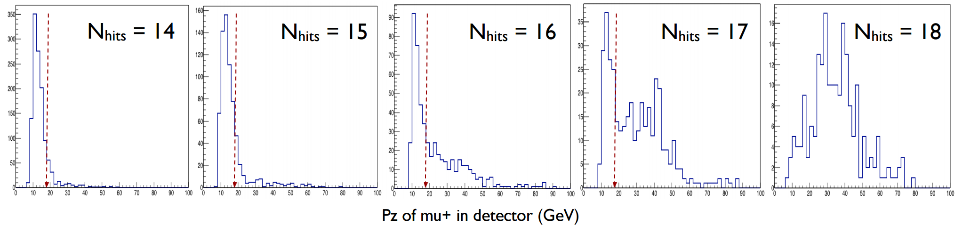
\includegraphics[width=\textwidth]{figures/analysis/likesign-pz-cut.png}
	\caption{The $p_z$ distribution of muons that form like-sign dimuon pairs, which is a source of background for DY signal events. In cases where $14\leq\text{numHits}<18$, imposing a cut on $p_z>$\unit[18]{GeV} removes a majority of this background.}
	\label{fig:likesign-pz-cut}
\end{figure}

\begin{table}
	\centering
	\ra{1.1}
	\begin{tabular}{@{}llll@{}} \midrule
		\textbf{Table} & \textbf{Value}  & \textbf{Good range} & \textbf{Type} \\ \toprule
kTrack & numHits & $>14$ & Quality \\
 & roadID & $\neq0$ & Quality \\
 & z0  & (-400, 200)  & Quality \\
 & chisq/(numHits - 5) & $<5$ & Quality \\
 & pz1 (Where numHits $\neq$ 18) & $>18$ & Quality \\
 & chisq\_dump - chisq\_target & $>10$ & Target \\ \midrule
kDimuon & dx & (-2, 2)  & Quality \\
 & dy & (-2, 2)  & Quality \\
 & dz & (-300, 200)  & Quality \\
 & dpx & (-3, 3)  & Quality \\
 & dpy & (-3, 3)  & Quality \\
 & dpz & (30, 120)  & Quality \\
 & xB & (0, 1)  & Quality \\
 & xT & (0, 1)  & Quality \\
 & xF & (-1, 1)  & Quality \\
 & trackSeparation & (-250, 250)  & Quality \\
 & chisq\_dimuon & $<15$ & Quality \\
 & px1 & $>0$ & Quality \\
 & px2 & $<0$ & Quality \\
 & dz & (-300, -60)  & Target \\
 & mass & $>4.2$ & Drell-Yan \\ \midrule
Event & MATRIX1 & 1 & Trigger \\ \midrule
kEvent & status & 0 & Quality \\ \midrule
QIE & $\forall$(RF+08, RF+07, \ldots RF-08) & $<$ Beam.Inh\_thres & Quality \\
 & $\forall$(RF$\pm XY$) & $>0$ & Quality \\
 & triggerCount & $\geq0$ & Quality \\
 & intensity\_p & $<60000$ & Quality \\
\bottomrule
\end{tabular}
\caption{A list of all quality and kinematic cuts for selecting good quality dimuons from the target.}
\label{tab:all-other-cuts}
\end{table}

\section{Normalization of Relative Yields}

The base measurement for the studies presented in this paper is, fundamentally, the number of dimuon events on a given target. This is known as the \emph{raw yield} (Y). The ratio of these yields for a given target is used to study the kinematic dependence of the \emph{per nucleon cross section ratio} that defines these phenomenon, but there must be a target-to-target normalization for such measurements.
\begin{equation}
R \equiv \frac{F_2^A}{F_2^D} \approx \frac{\sigma_{\mu\mu}^A}{\sigma_{\mu\mu}^D} \frac{2}{A} = N_{A/D} \frac{Y^A}{Y^D}
\end{equation}
Here, $A$ is the mass number of the target nucleus, and $N_{A/D}$ is the normalization factor, which can be expressed as:
\begin{equation}
	N_{A/D} =
		\left(\frac{ N_0^D \cdot \text{lt}^D \cdot T^D(\xi)}{N_0^A \cdot \text{lt}^A \cdot T^A(\xi) } \right) \cdot 
		\left( \frac{ 2 \cdot n_D \cdot L^D }{ A \cdot n_A \cdot L^A } \right) \cdot 
		\frac{ \varepsilon^D }{ \varepsilon^A }  \cdot 
		\frac{ \bar{\Omega}^D }{\bar{ \Omega}^A } \cdot 
		\frac{ \epsilon^D }{ \epsilon^A }
\end{equation}
where $N_0$ is the number of incident protons, \emph{lt}$^A$ is the \% live time on the target, $T^A$ is the target transmission (or beam attenuation) factor, $n_A$ is the number of nuclei per unit volume, $L^A$ is the target thickness, $\varepsilon^A$ is the detector efficiency, $\bar{\Omega}^A$ is the spectrometer acceptance, and $\epsilon^A$ is the tracking reconstruction efficiency. One of the key benefits of performing a ratio measurement is that, to good approximation, the terms regarding chamber efficiency, tracking efficiency, and acceptance should be equal across targets and should therefore cancel each other out. How well this assumption holds up will be assessed and evaluated.

With the normalization applied, this ratio $R$ can be accurately studied by being binned in one or more kinematics in order to observe interesting behaviors and compare them against previous measurements and various models. Once The cuts described in the previous section are applied, the surviving dimuons are all considered to be \emph{good quality target Drell-Yan dimuons}, and all analyses and corrections described from here on refer to them only.

This section will discuss the several components of the target-to-target relative normalization from the determination of beam intensity, target thickness, live time, chamber efficiency, and acceptance. Beam intensity and live time information was obtained from the BIM and scaler data. Acceptance was calculated with Monte Carlo simulation. Finally, chamber efficiencies and their ratios per target were studied with NIM3 random trigger data embedded onto clean MC. The tracking efficiencies are highly rate-dependent, and will be discussed at length in another section.

\subsection{Live Proton Count and Beam Attenuation}

The measurements of the number of incident protons, live time, and beam attenuation combine to give a figure for the total number of protons on target for which data was recorded. The important sources to consider here are the upstream SEM detectors that record the number of incident protons, the QIE recorded sums of protons (in QIE units), the number of QIE units for which there was either a trigger inhibit or DAQ deadtime. In practice, SeaQuest calculates a value called ``live protons'' \emph{for each spill}:
\begin{equation}
 N_0^A = \text{G2SEM}\ \ \ ;\ \ \ \text{lt}_A = 
 \frac{\text{QIESum} - \text{inhibit} - \text{deadtime}}{\text{QIESum}}\ \ \ ;\ \ \ 
 liveProton = N_0^A \cdot \text{lt}_A
\end{equation}
this \emph{liveProton} value is integrated, good spill by good spill, for every target in each data set.

\red{What are average livetimes for the experiment? Deviations?}

It is also important to factor in the effects of inelastic scattering of the beam within the target, causing the effective amount of beam-on-target to decrease with every step $dz$ through the target. This is different for each target based on target nuclear densities and cross sections. With this, the liveProton value can be corrected. Consider incident proton number $N_0$, where $dN$ is the number of protons attenuated when passing through target slice $dz$, and $L$ is the total length of the target. The function for the number of protons remaining at a given position $z$ is
\begin{equation}
 N(z) = N_0 e^{-\frac{\rho_A}{\text{NIL}_A} z} = N_0 e^{-z/\lambda}
\end{equation}
where $\rho_A$ is the density of the material, $\text{NIL}_A$ is the nuclear interaction length of the target, and $\lambda = \frac{\text{NIL}_A}{\rho_A}$. When integrating over the length of the target, one arrives at the total [$\text{protons}\cdot \text{cm}$] exposed to the target. Assuming that each proton interacts independently, one can divide this integral by the length of the target to arrive at \emph{effective} number of protons incident on the target
\begin{equation}
N_{\text{eff}} = \frac{1}{L} \left[ N_0 \lambda (1 - e^{-\frac{L}{\lambda}})\right] = N_0 \left[\frac{1 - e^{-\xi}}{\xi}\right] =  N_0 T(\xi)\ \ \ ;\ \ \ 
\xi = L/\lambda.
\end{equation}
The normalization of the transmission or beam attenuation factor $T^D/T^A$ is therefore only a function of the length of the target, its density, and its nuclear interaction length. In total, the product of $N_0 \cdot \text{lt} \cdot T(\xi)$ represents the effective protons on target which was recorded by the data acquisition systems. Values of $\xi$ and $T(\xi)$ can be found in Table~\ref{tab:targ-details}.

\subsection{Target Density Ratios}

The number of nucleons that the effective protons will interactive should be considered when performing the target-to-target normalization. Aside from the background ``targets'' and liquid hydrogen, there are four nuclear targets in this A-dependence study. The nucleons in liquid deuterium are viewed as essentially free particles, and therefore proved an isoscalar reference by which the heavier targets are compared to. In all, the nuclear targets used are $D_2$, C, Fe, and W, and their attributes pertinent to target density ratios can be found in Table~\ref{tab:targ-details}. The yield ratios are normalized to the number of nucleons in each target by the normalization component $(2 \cdot n_D \cdot L^D) / (A \cdot n_A \cdot L^A)$. 

\begin{table}
	\centering
\begin{tabular}{lrrrrrrrr}
	\toprule
	{} &  Target &  Length[cm] & $n_A$ [mol/cm$^3$] & $\rho$ [g/cm$^3$] &  NIL [g/cm$^2$] &   $\lambda$ [cm] & $\xi$ & T($\xi$) \\
	Target & Position & & & & & & & \\
	\midrule
	$D_2$ & 3 & 50.80 & 0.081 & 0.163 & 71.8 & 439.41 & 0.1156 & 0.944 \\
	Fe & 5 & 1.91 &	0.141 & 7.874 & 132.1 & 16.78 & 0.1136 & 0.945 \\
	C & 6 & 3.32 & 0.150 & 1.802 & 85.8 & 47.61 & 0.0698 & 0.966 \\
	W & 7 & 0.95 & 0.105 & 19.300 & 191.9 & 9.94 & 0.0958 & 0.954 \\
	\bottomrule
\end{tabular}
\caption{Details pertaining to the measurables and physical properties individual nuclear targets.}
\label{tab:targ-details}
\end{table}

\red{Uncertainties in densities, target lengths? Find solid target with largest uncertainty, estimate LD2 uncertainty the best we can, get \% systematic from the ratio of them.}

\subsection{Detection Efficiency}

The key cause of detector inefficiency is high occupancies from high intensity events. Also, the total number of tracks that fired off elements of the many detectors is dominated by events generated from the \unit[503]{cm} iron beam dump. The difference in interaction lengths of the targets should have only a small effect on the absolute chamber and hodoscope efficiencies. Further, any longer term time-dependent drifts in detector efficiencies will largely cancel out due to the frequent minute-by-minute interchange of targets. It is therefore justifiable to assume that there is no target-to-target chamber efficiency dependence to normalize to. The overall ratio of detector efficiencies between targets is therefore taken to be $\varepsilon^D/\varepsilon^A=1$. 

It is however possible that pions created in the targets have more of a chance to decay into muons that proceed to add to the background hit rates of the experiment; pions created in the beam dump are much more likely to get re-absorbed before they decay. To investigate the possible magnitude of this contribution to occupancy, detector occupancies were studied for the different targets in unbiased NIM3 random events as a function of chamber intensity. We see in Figure~\ref{fig:occ-int-targ} that they are not significantly different from each other, though there is a slight difference in occupancies between the deuterium target and the rest. However, since the occupancy distributions at a given intensity bin do not change much for a given intensity, it is safe to assume that the efficiencies likewise do not change by much from target-to-target.
\begin{figure}
	\centering
	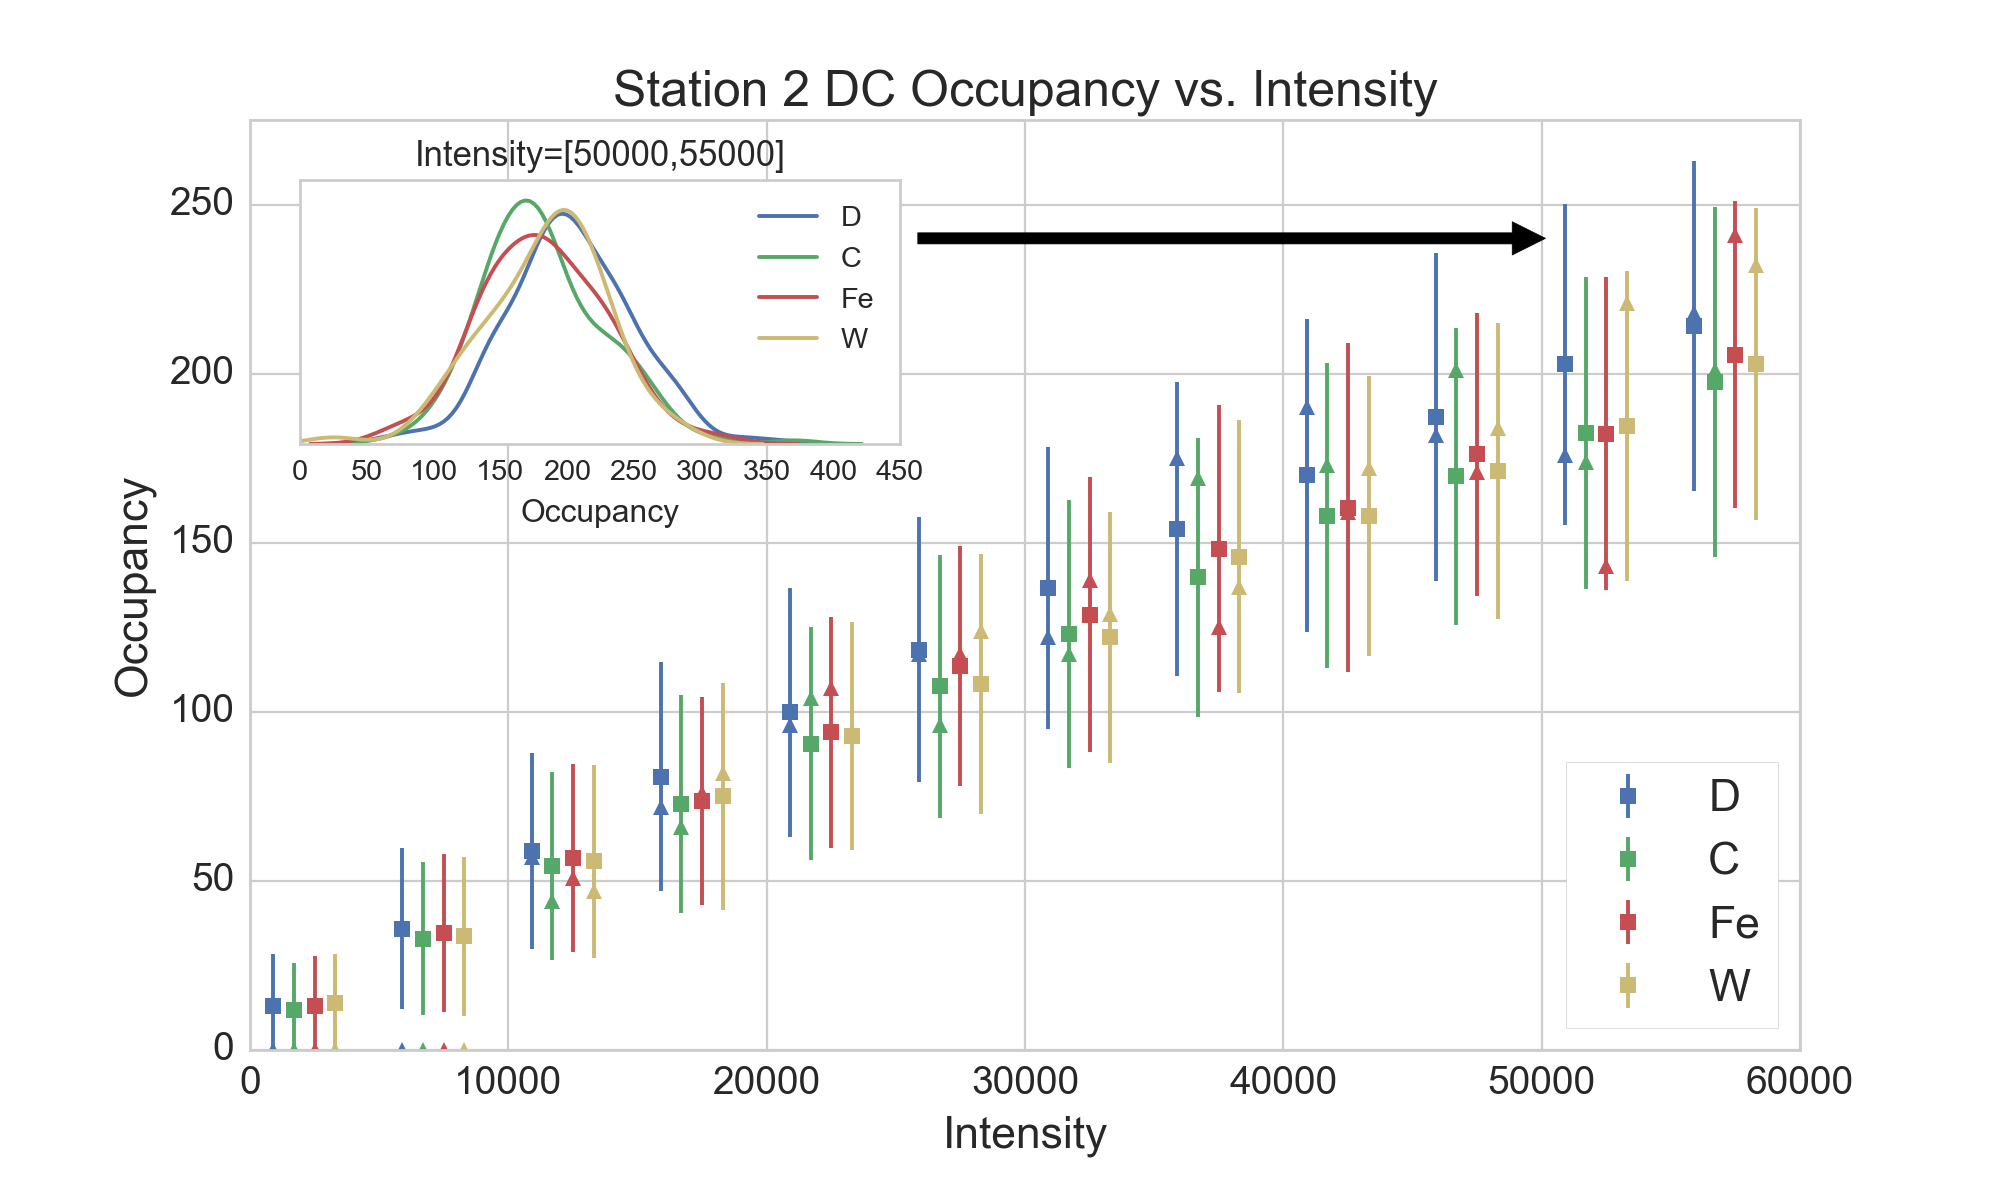
\includegraphics[width=5in]{figures/analysis/targ-occupancy.png}
	\caption{The Station 2 drift chamber occupancy for the four targets as a function of intensity. The error bars show a systematic deviation of occupancies from the mean for a given intensity bin. The inset plot shows the distributions for the intensity bin in which the values differ the most. The triangle markers represent the modes of the distributions.}
	\label{fig:occ-int-targ}
\end{figure}

To override any concern of chamber efficiencies having an effect on any absolute or ratio measurements, a study was performed to measure the effect of chamber efficiencies on the track reconstruction algorithm. This was done by embedding clean Monte Carlo-generated Drell-Yan dimuons into real NIM3 random event hit data. Then, a constant 94\% chamber efficiency was applied by removing a random 6\% of the chamber hits, and tracking was performed on this sample. The 94\% figure reflects the best estimate of overall chamber efficiencies at SeaQuest. Following that, a rate-dependent chamber efficiency was imposed of the form
\begin{equation}
\varepsilon(I) = 0.95 - a \cdot I
\end{equation}
where $a$ was set to \unit[2e-6]{protons$^{-1}$}. This resulted in a linear drop in efficiency with it dropping to as low as 75\% at the highest intensity regions considered (\unit[100000]{protons}). The tracking algorithm was then run on this data sample.
	
For even the constant 94\% efficiency case, the tracking is expected to decrease in \emph{tracking efficiency} (a very different topic to tackle, as we will approach later in this chapter) as intensity increases and pattern recognition becomes more difficult as overall occupancies increase. The important to observation to make is how this intensity-dependent tracking efficiency compares to the case of decreasing efficiency. For both cases, the ratio of successful reconstructions to all thrown dimuons (before even the trigger acceptance is imposed) can be seen in Figure~\ref{fig:ktrack-eff-int}. It is perhaps surprising to see that even at high intensities, the linear drop in tracking efficiencies does not change between the two cases. The reason for this is due to the fact that the tracking algorithm is very \emph{robust} in the way it is able to handle missing hits, as it only requires a few hits in each station (3 out of 6) to successfully find a track.
\begin{figure}
	\centering
	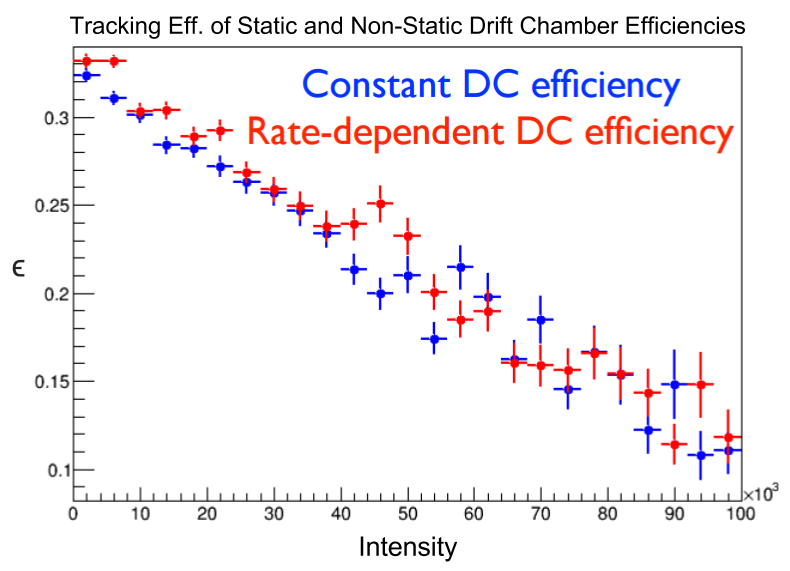
\includegraphics[width=4in]{figures/analysis/ktrack-eff-int.png}
	\caption{The ratio of successful reconstruction to all thrown by MC for two chamber efficiency models. The linear decreases in efficiency are not significantly different from each other.}
	\label{fig:ktrack-eff-int}
\end{figure}

Putting this together:
\begin{itemize}
	\item Differences in chamber efficiency between targets could only come from different resultant chamber occupancies as a result of that target being in the beam's path.
	\item Chamber occupancies are only slightly different for deuterium when compared to the other nuclear targets, and so if efficiencies are different between targets, the modification will likely be very small.
	\item Even in the case of vastly different efficiencies, the tracking efficiency is unchanged.
	\item As a result, effect of chamber efficiency on the yields will be the same for all targets.
	\item Therefore, $\varepsilon^D/\varepsilon^A$, a measure of how the chamber efficiency effects the deuterium target yields as compared to a nuclear targets, can be considered to be 1.
\end{itemize}

\subsection{Relative Acceptance Correction}

The target dependence of the acceptance was studied via Monte Carlo of yield ratios of heavy targets to that of deuterium for the valid kinematic regions of the experiment. These regions are \unit[4.2]{GeV}$<M_{\gamma^*}<$\unit[10]{GeV}, $0.08<x_2<0.5$, $XX<x_F<YY$, and $XX<p_T<YY$. Since no nuclear effects are simulated by the Monte Carlo generator, this ratio should lie at 1; any deviation of this must be purely from the acceptance effects due to the slight differences in the geometries of the targets. The results can be seen in Figure~\ref{fig:targ-acceptance}.
%\begin{figure}
%	\centering
%	\includegraphics[width=5in]{figures/analysis/targ-acceptance.png}
%	\caption{Ratios of accepted dimuons from heavy targets to deuterium for all kinematic regions of interest.}
%	\label{fig:targ-acceptance}
%\end{figure}
The acceptances of solid targets were calculated by MC to be Z.ZZZ larger than that of the liquid deuterium target. As such, a correction factor of $\bar{\Omega}^A/\bar{\Omega}^D = Z.ZZZ$ is included in the target-to-target normalization.

\section{Dimuon Weights and Corrections}

Weighting of events is a standard procedure for mapping one distribution onto another. The most common example is with Monte Carlo (MC) simulation weighting. A simple physics event MC meant to simulate a well-defined process will `throw' an event with certain kinematics randomly drawn from known distributions via \emph{inverse transform sampling}. By doing this, the simulation is already close to being physical, but according to the cross section of a given process, a certain combination of kinematics will be decidedly more or less probable. A weighting subroutine calculates this likelihood for each event and assigns a weight with respect to how likely that event is based on the kinematics thrown. When binning this weighted data, the adjusted number of events in a bin is given by
\begin{equation}
	N_{bin} = \sum_{i \in bin} w_i\ \ ;\ \ \sigma_{bin} = \sqrt{\sum_{i\in bin} w_i^2}
	\label{eq:gmc-weight}
\end{equation}
which reduces to the Poissonian statistical picture when all weights are 1.

Weighting in this manner can be used in any case where it is desirable to map one distribution to another, as in the case of applying corrections in the case of efficiencies and background subtractions. The most intuitive connection between the use of weights and corrections is in the case of efficiency corrections. Let us say that a dimuon with a certain set of kinematics, for whatever combination of effects, has a reconstruction efficiency of 80\%. This means that four out of five actual dimuons with these kinematics will be reconstructed. If you know this efficiency $\epsilon_{recon}$, you can apply a weight as $w = 1/\epsilon_{recon}$ to each dimuon, as each dimuon represents, in part, a larger population that is not fully represented. In the case of our example, a single dimuon represents $1/0.80 = 1.25$ dimuons in order to make up for the ones that are missed due to that specific inefficiency.

At SeaQuest, there is an issue of rate dependence, and as the sources of this effect is identified, we apply a correction for each source in the form of an applied weight. Here, we discuss the reconstruction efficiency and empty/none target background subtraction corrections.

\subsection{``kEfficiency'' Correction Using Messy/Clean Data}

It is a matter of combinatorics at SeaQuest that, as the intensity increases, the number of background hits on all of the detectors increases. As the number of hits in all the detectors increases, the harder it become for the tracking to identify the actual dimuon(s) from the whole event. This is regarded to be an intensity-dependent tracking efficiency. Seeing as the primary tracking algorithm for SeaQuest is kTracker, this is known as the ``kEfficiency'', and its intensity, target, and kinematic dependency makes it a factor to model and correct for.

The procedure developed by Evan McClellan of UIUC for calculating this kEfficiency is to take compare the performance of the tracking on a clean MC sample of dimuons to an analogous sample that's mixed in with real intensity-dependent background. To do this, a \emph{single} sample of MC-generated dimuons and all of their hits is generated; this sample is denoted as the \emph{``clean''} sample. Then, this sample is mixed with all of the hits from a NIM3 event from the experimental data. The NIM3 trigger, as is discussed in Chapter~2, is the randoms trigger, and by using these events we avoid any effects due to trigger selection bias. This mix of MC dimuons and NIM3 triggered data is denoted as the \emph{``messy''} sample. These NIM3 events all have an intensity, and by embedding a clean MC dimuon into a situation typical of an event at a given intensity, we get a basis by which to judge how efficiently the tracking can reconstruct a dimuon in the clean sample versus the messy sample as a function of intensity (and other kinematic variable).

It is important to note that the DY cross section is so small that there is a negligible chance that a given randomly-triggered NIM3 event will contain an actual dimuon, nonetheless a dimuon matching the characteristics of the MC dimuon that is embedded. As such, it is assumed that the dimuon embedded in the NIM3 event is the only dimuon to find in the event. It is also justified to assume that the kinematics of a dimuon is in no way correlated to the intensity, and the intensity of an event relates only to the amount of background hits observed. The relation to the intensity and the number of background hits can be observed in Figure~\ref{fig:NIM3-Int-Mult}.

\begin{figure}
	\centering
	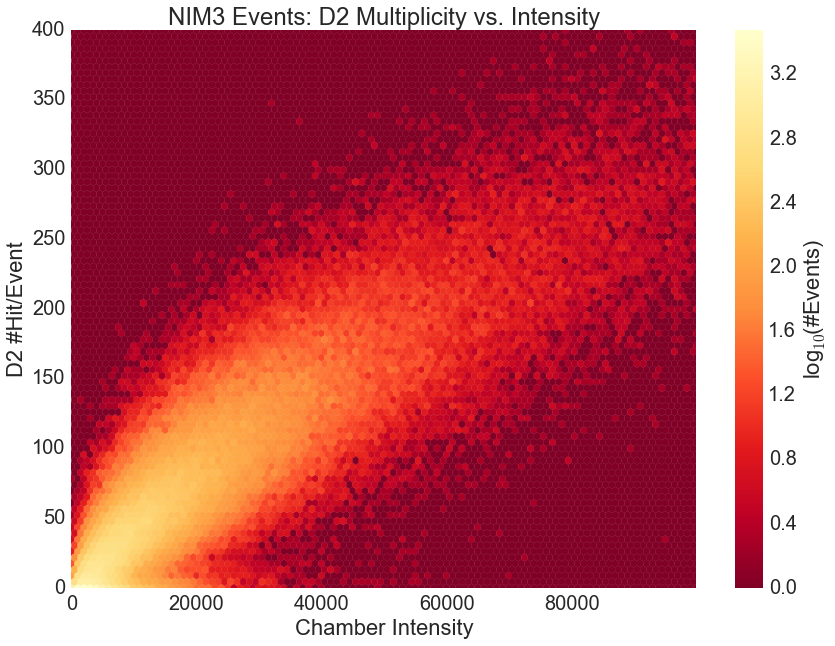
\includegraphics[width=4in]{figures/analysis/NIM3-Int-Mult.png}
	\caption{The linear tendency of detector multiplicity to increase with intensity is observed by looking to unbiased NIM3 events. Here, the occupancy per event of the drift chambers at station 2 are shown as a function of intensity.}
	\label{fig:NIM3-Int-Mult}
\end{figure}

Once the messy and clean samples are prepared, the tracking software is run on them and the two outputs are compared. The first step is to bin the resulting reconstructed dimuons into intensity bins. This binning uses the weights of the dimuons that is assigned by the GMC that created them. The weights are used instead to avoid undue influence on the efficiency from dimuons that are highly unlikely to occur. The value of the bin and its uncertainty are calculated according to Eq.~\ref{eq:gmc-weight}.

For each matching bin, the ratio of $\frac{\#messy}{\#clean}$ values is used to calculate the efficiency of the tracking for that bin. The uncertainty of that efficiency is more complicated, as the relation between the messy and clean samples is of a \emph{binomial} nature. Each dimuon successfully reconstructed in the messy sample represents a \emph{positive} outcome from the number of possible outcomes which is represented by the clean sample. With this kind of relationship, binomial uncertainty calculations must apply. For large enough N number of trials and efficiency $\epsilon\notin \{0,1\}$,
\begin{equation}
\epsilon = \frac{N_+}{N}\ \ ;\ \ \delta\epsilon = \sqrt{\frac{N_+ N_-}{N^3}} = \sqrt{\frac{\epsilon(1-\epsilon)}{N}}
\label{eq:binomial-naive}
\end{equation}
but when weighted trials are involved, things become more complicated in calculating the statistical error. The calculation of this statistical error\cite{blist:binomial} is as follows:
\begin{eqnarray}
	\epsilon & = & \frac{\sum\limits_{i\in+}w_i}{\sum\limits_i w_i} \\
	\delta\epsilon & = & \frac{\sqrt{\sum\limits_{i\in+} w_i^2 \left(\sum\limits_{i\in-} w_i \right)^2 + \
			\sum\limits_{i\in-} w_i^2 \left(\sum\limits_{i\in+} w_i \right)^2}} {\left(\sum\limits_{i}w_i\right)^2}
	\label{eq:binomial-weighted}
\end{eqnarray}
where
\begin{eqnarray}
\sum\limits_{i\in-} w_i & = & \sum\limits_{i\in+}w_i - \sum\limits_{i\in+}w_i \\
\sum\limits_{i\in-} w_i^2 & = & \sum\limits_{i\in+}w_i^2 - \sum\limits_{i\in+}w_i^2 
\end{eqnarray}

For a set of efficiencies, a linear function is fit to the efficiencies. This fit function would then be used to calculate the efficiency for any given dimuon that occurs at any given intensity. The linear parameters are fitted to the data (which is weighted by its statistical uncertainties) by a $\chi^2$-minimization procedure to render a line of best fit along with a confidence interval (Fig.~\ref{fig:keff-all})

\begin{figure}
	\centering
	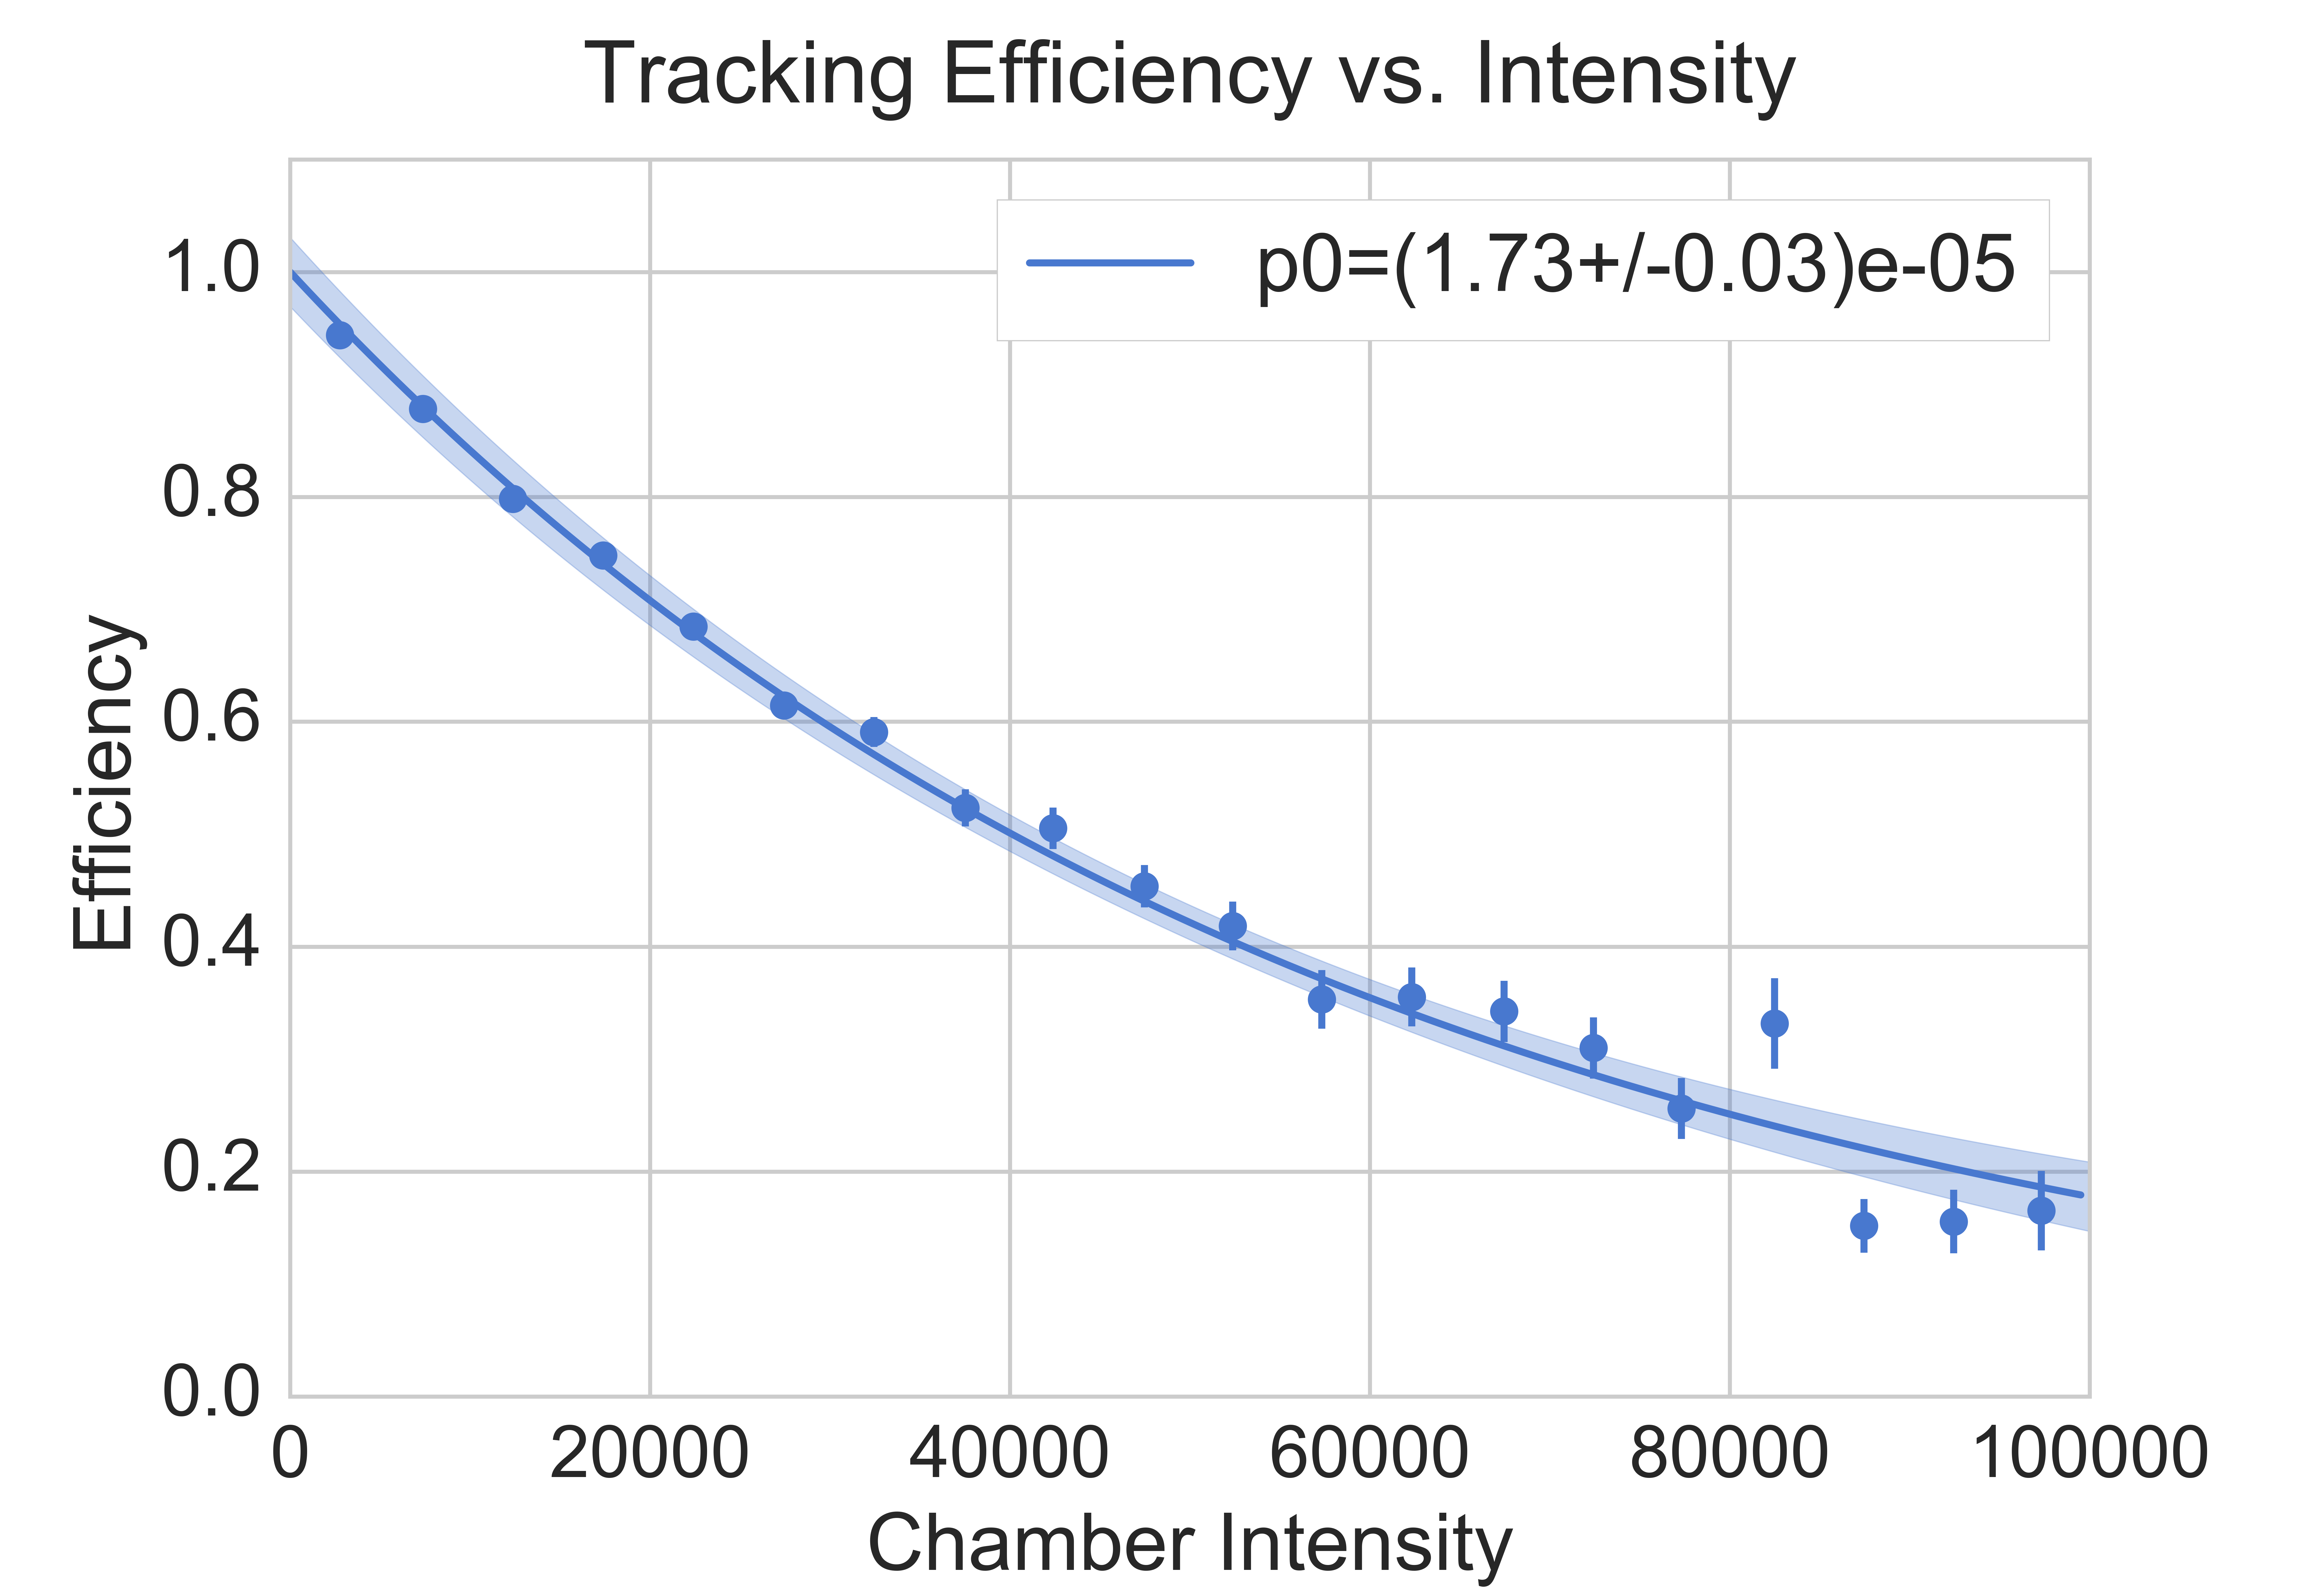
\includegraphics[width=4in]{figures/analysis/all-keff-int.png}
	\caption{The ratio of ``messy'' to ``clean'' dimuon samples from the Deuterium target in Roadset 67 data. This shows the linear relationship of the tracking efficiency to the intensity of the events. The shaded band indicates the 95\% confidence band of the fit.}
	\label{fig:keff-all}
\end{figure}

Further, these fits have a statistically significant kinematic dependence, so it becomes important to unfold the kinematic space and perform this procedure for several kinematic bins in one or more dimensions to assure an accurate efficiency calculation. Of the six defining kinematics of the dimuon, we examine the dependence of the fit on five of them: ($x_1, x_2, p_T, \theta, \phi$), neglecting the azimuthal production angle $\phi_{\gamma^*}$. Each of these five kinematics is divided into three bins (low, medium, high) values to observe on which kinematics the linear fit depends. The results are shown in Figure~\ref{fig:keff-all-kin}.
\begin{figure}
\centering
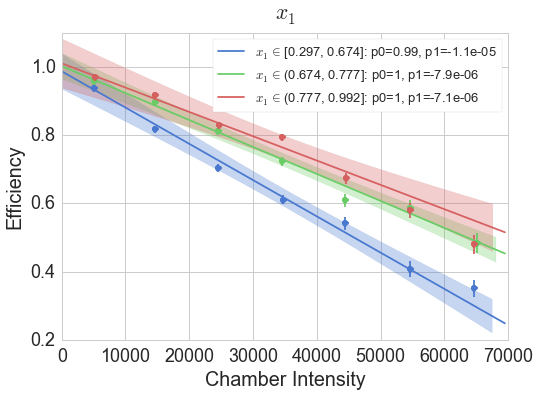
\includegraphics[width=0.49\textwidth]{figures/analysis/x1-keff-int.png}
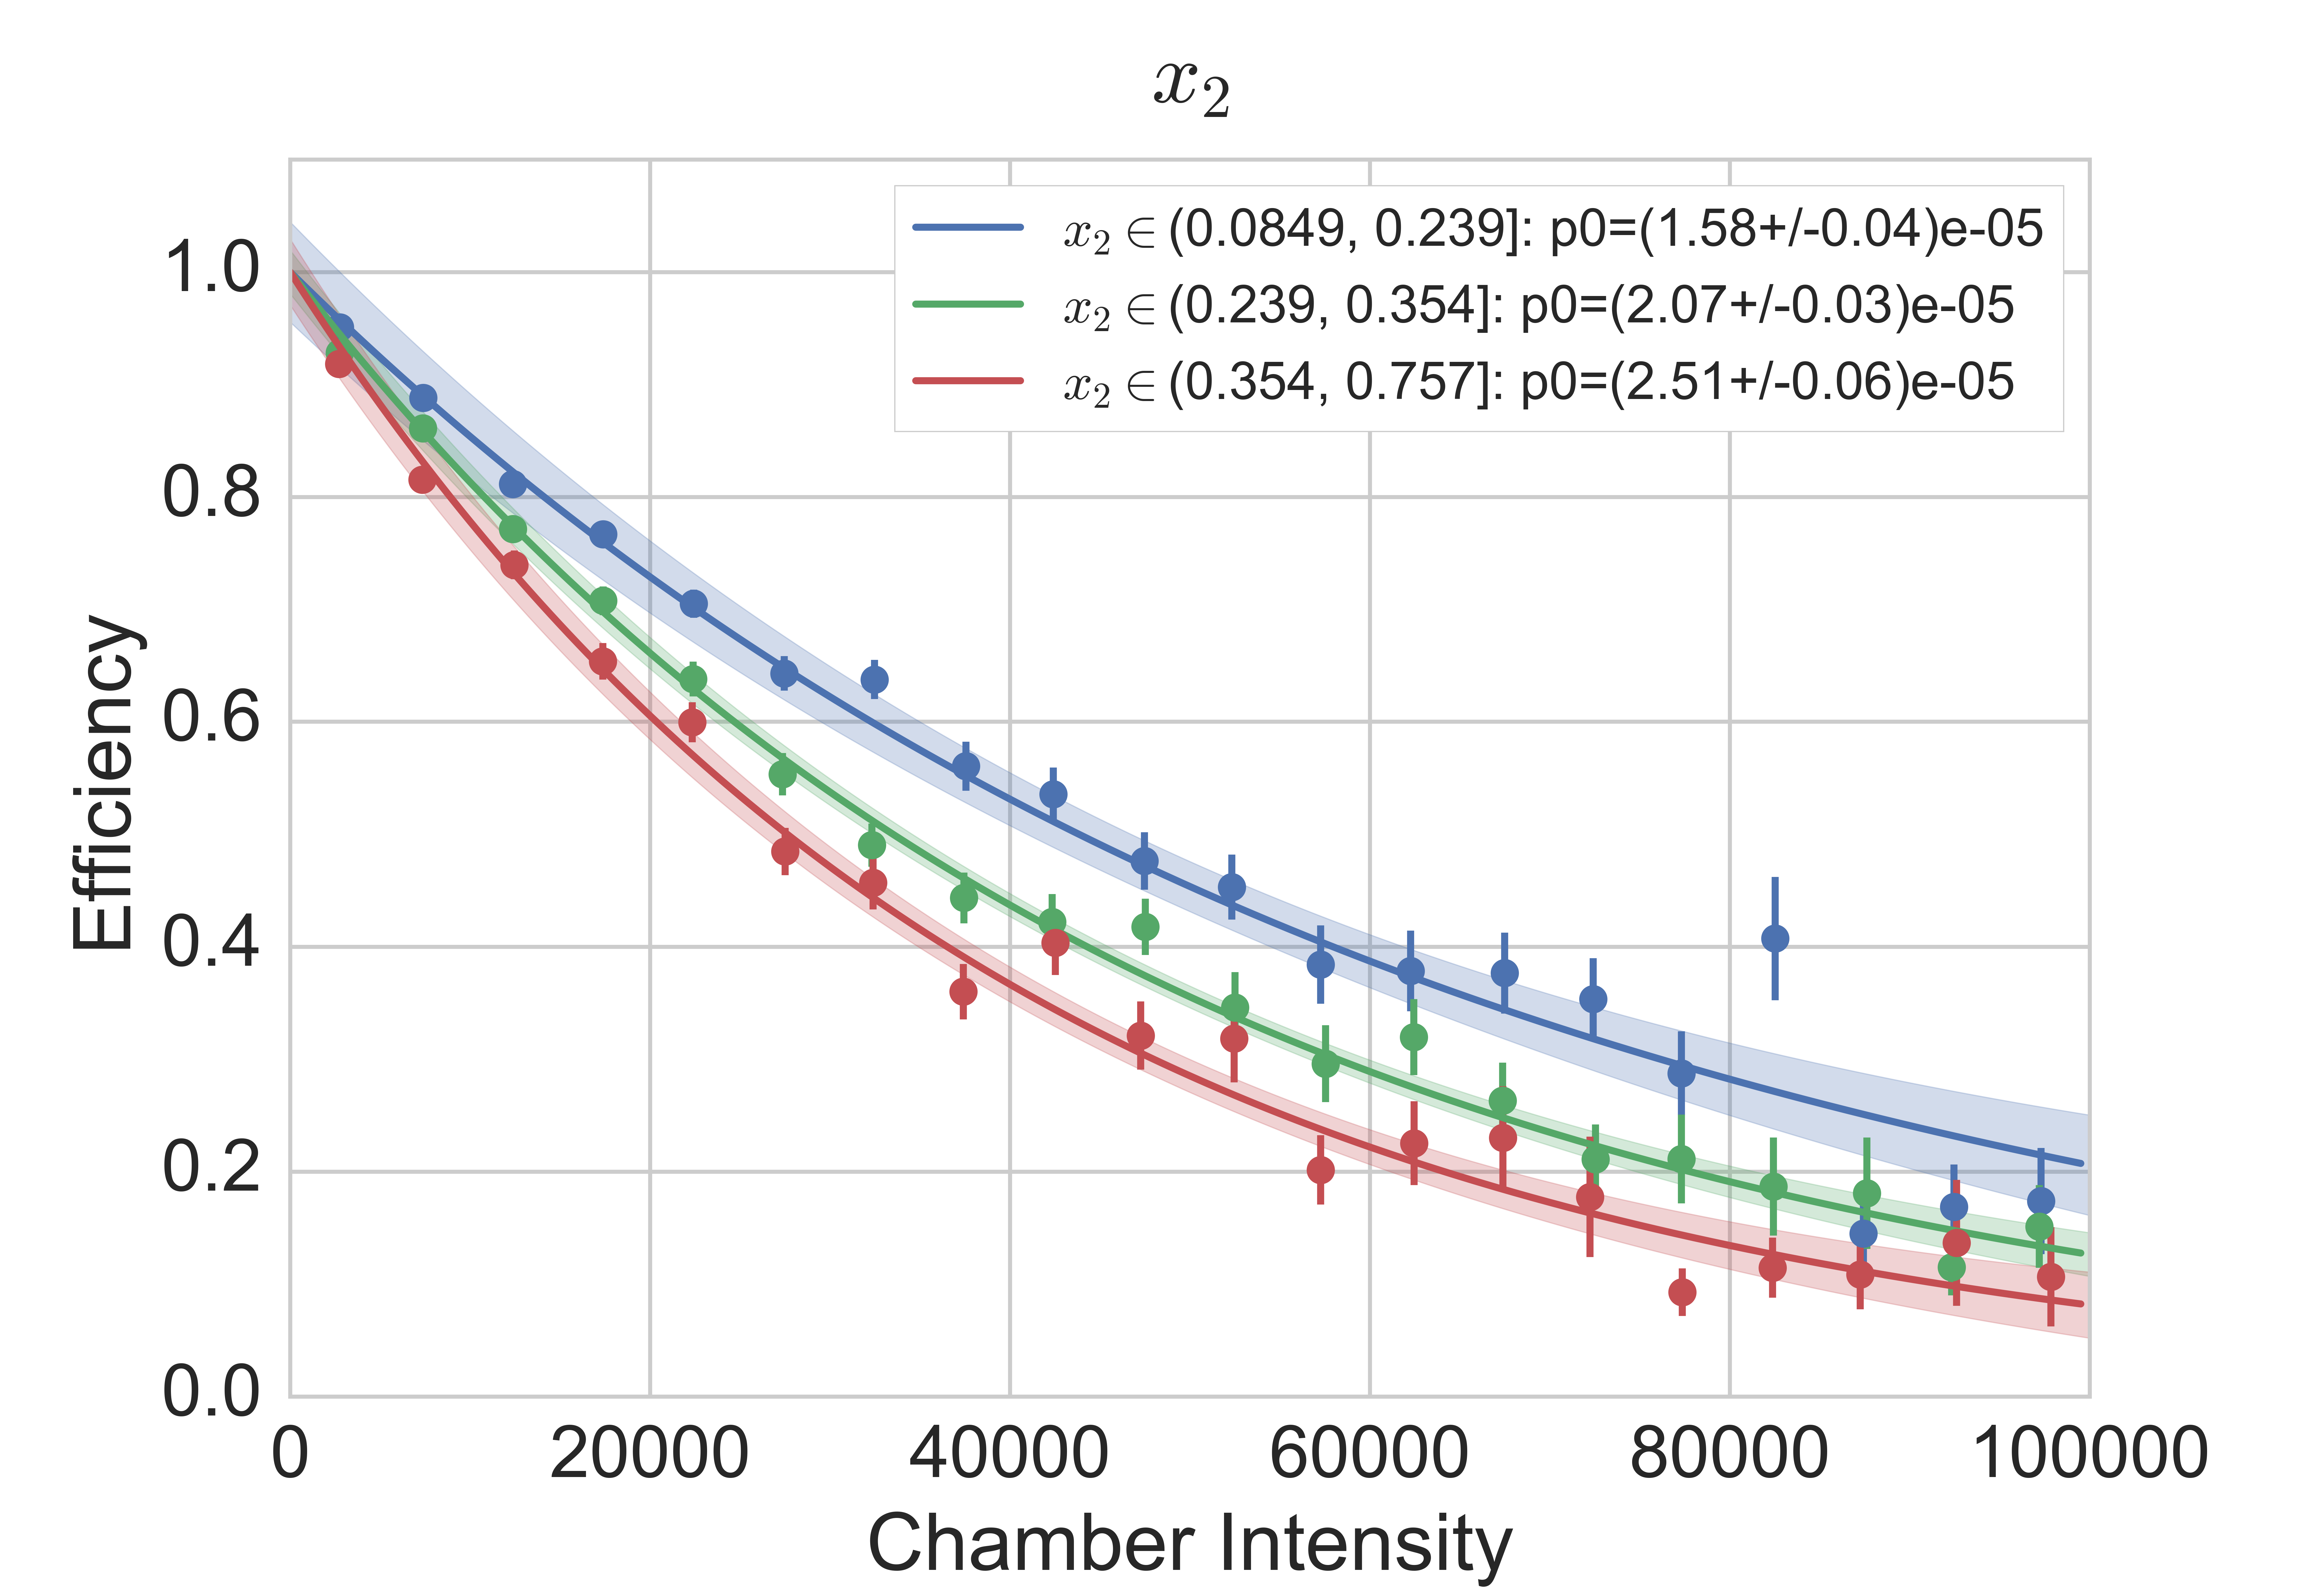
\includegraphics[width=0.49\textwidth]{figures/analysis/x2-keff-int.png} \\ \vspace{20px}
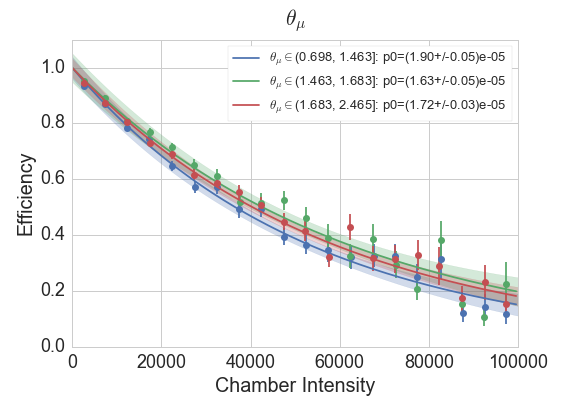
\includegraphics[width=0.49\textwidth]{figures/analysis/theta-keff-int.png}
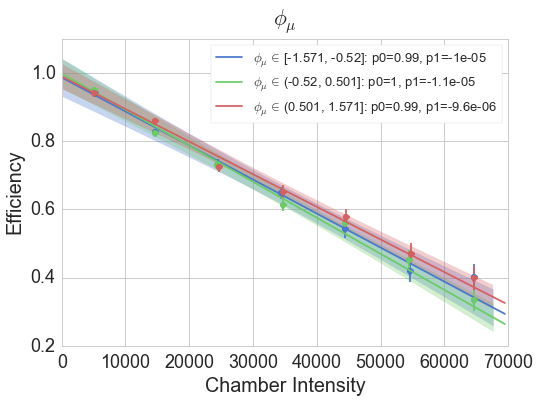
\includegraphics[width=0.49\textwidth]{figures/analysis/phi-keff-int.png} \\ \vspace{20px}
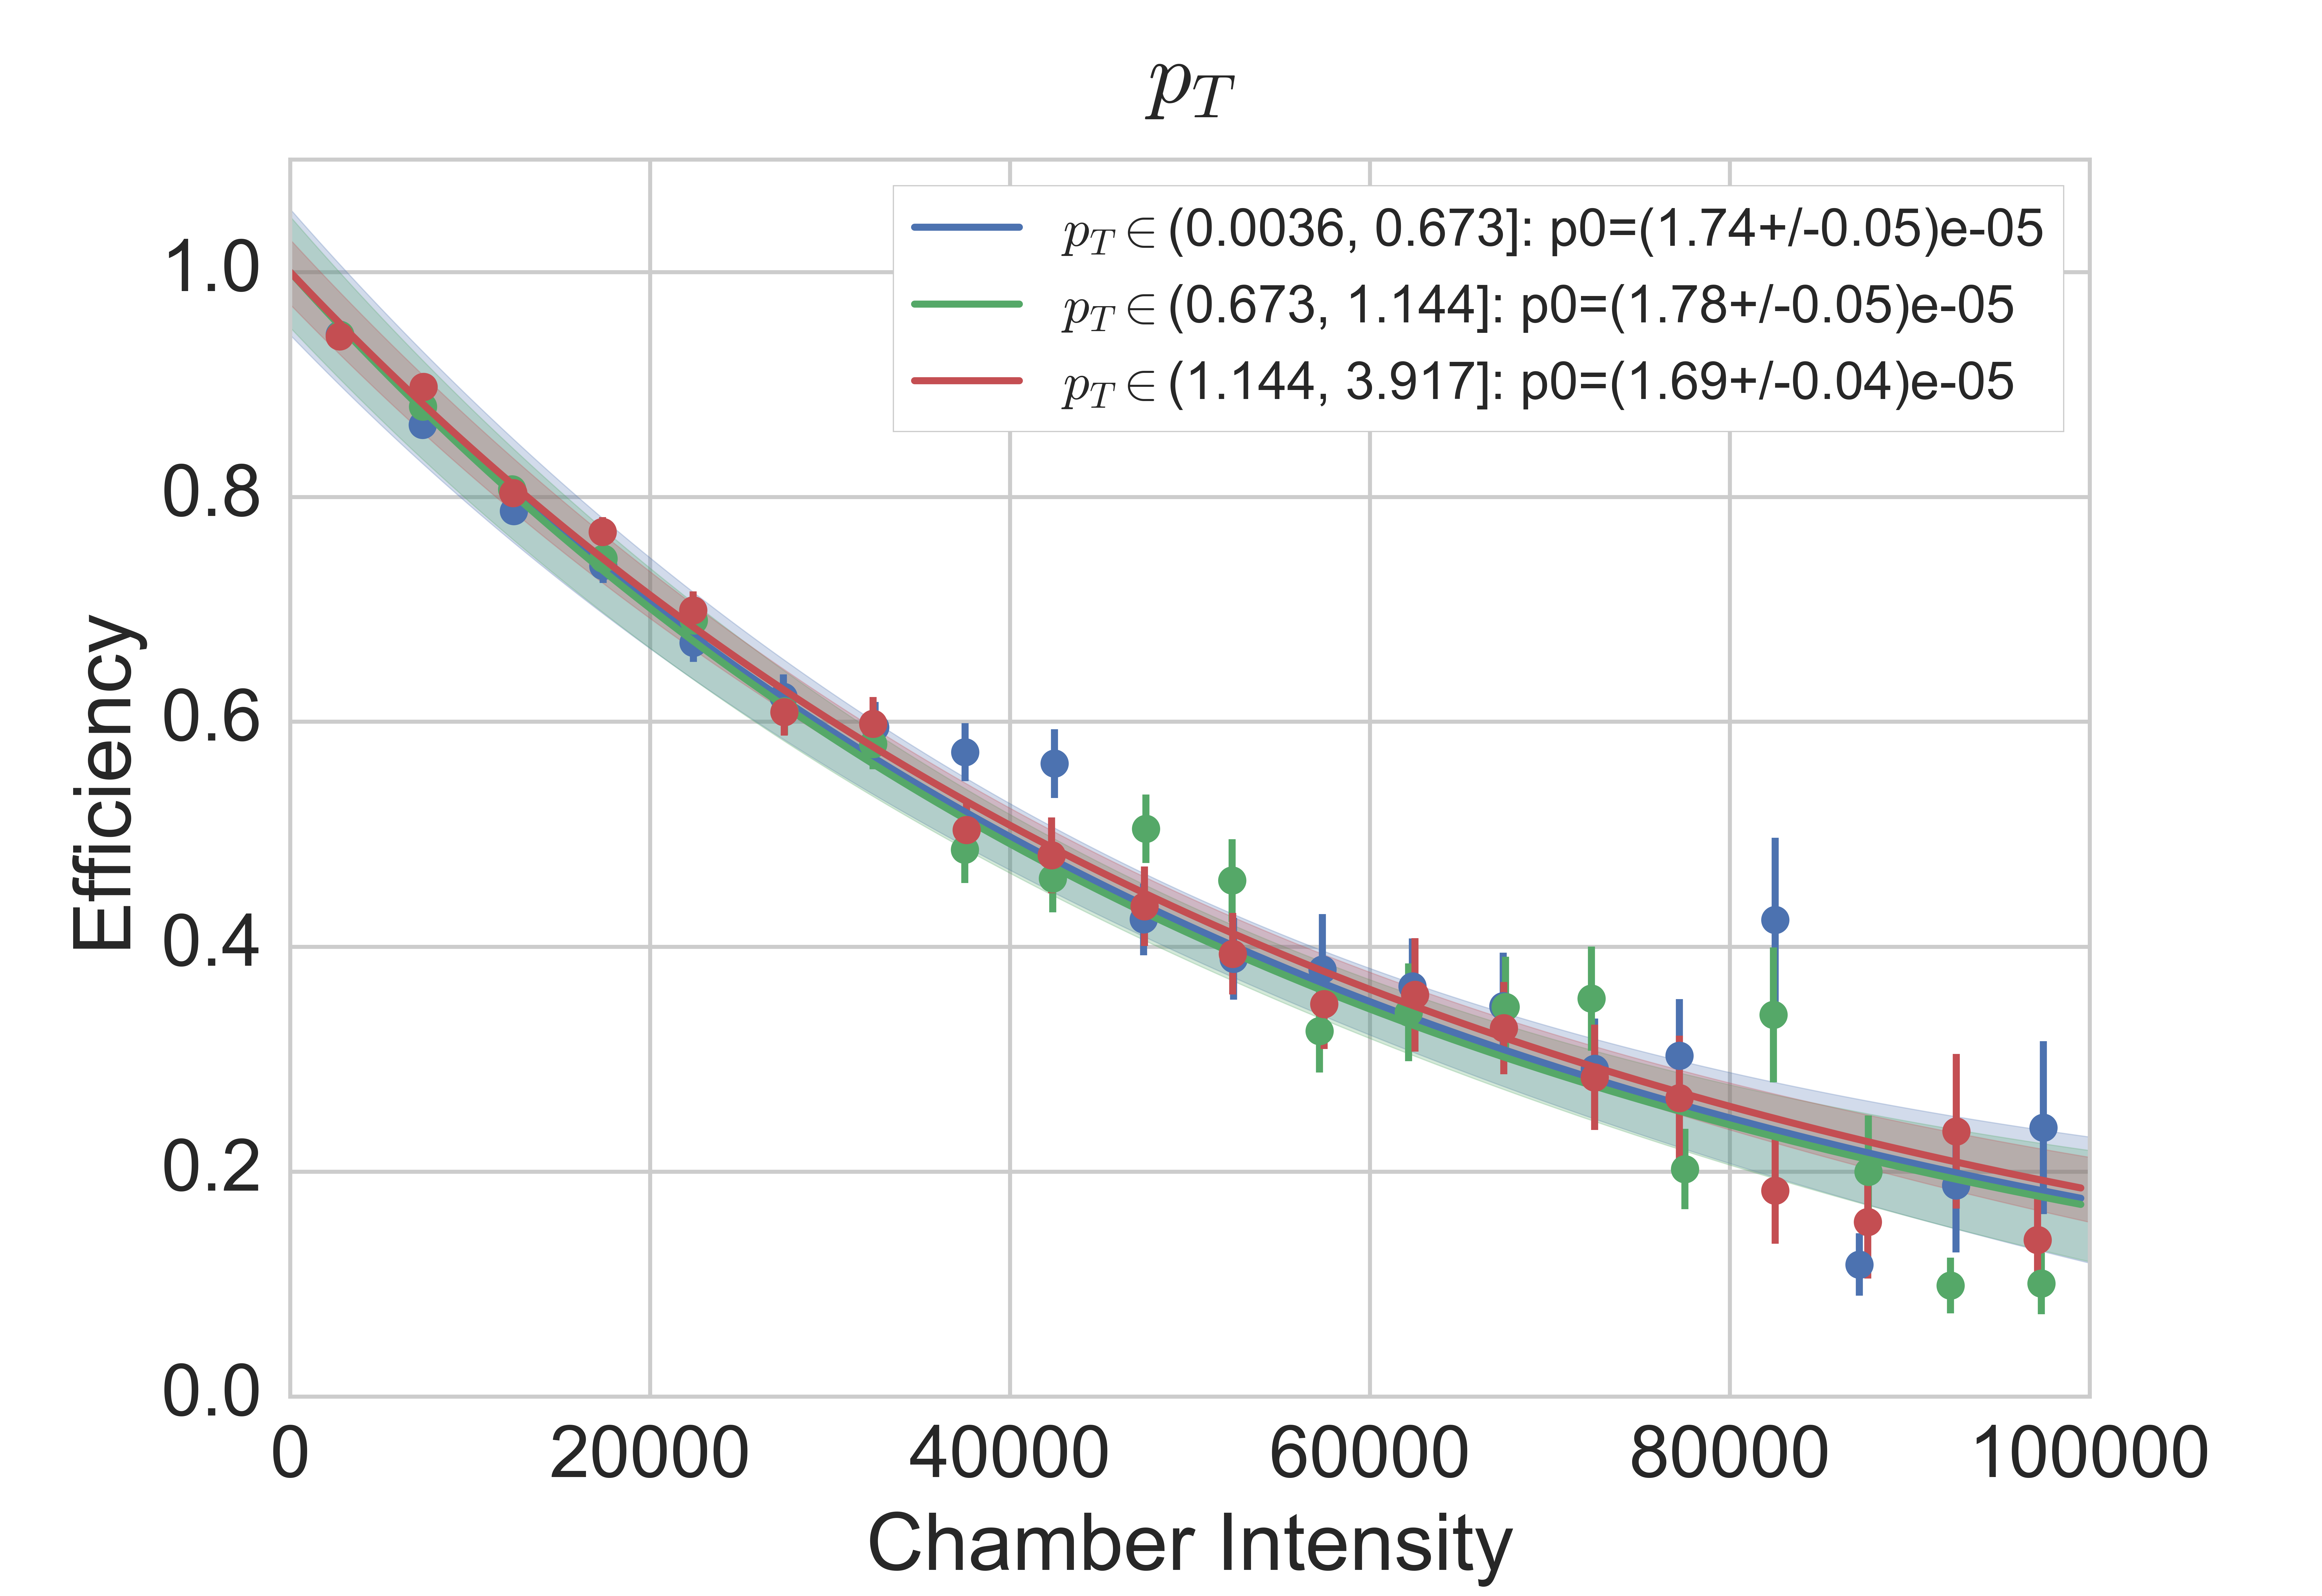
\includegraphics[width=0.49\textwidth]{figures/analysis/pt-keff-int.png} \vspace{10px}
\caption{Tracking efficiency with the data broken into three statistically equivalent bins in the five primary kinematics, ($x_1, x_2, \theta_\mu, \phi_\mu, p_T$). There appears to be a significant kinematic dependence on $x_1$ and $x_2$.}
\label{fig:keff-all-kin}
\end{figure}
The curves produced seem to indicate that there only exists a kinematic dependence on the $x_1$ and $x_2$ kinematics. If this is the case, then the clean and messy samples can be split two-dimensionally in these two kinematics, and a fit can be made to both variables. When analyzing dimuons, its kinematics can indicate which fit to use to calculate the tracking efficiency based on the intensity of the event, and a weight can be calculated.

But before we come to any clear conclusions, let us investigate two more kinematic phase spaces. We know from the discussion in Chapter 1 that \{$x_1, x_2$\} can be used almost interchangeably with \{$x_F, M_{\gamma^*}$\}, and each of $x_1$ and $x_2$ depend on both $x_F$ and $M_{\gamma^*}$. As such, if only one and not the other shows to influence the tracking efficiency curves, then only that one would be needed for the tracking efficiency correction. We see the behavior of the efficiency curves as a function of $x_F$ and $M_{\gamma^*}$ in Figure~\ref{fig:keff-mass-xf}. It can be concluded that since there is no substantial mass dependence observed, the tracking efficiency has a kinematic dependence solely on $x_F$.

\begin{figure}
	\centering
	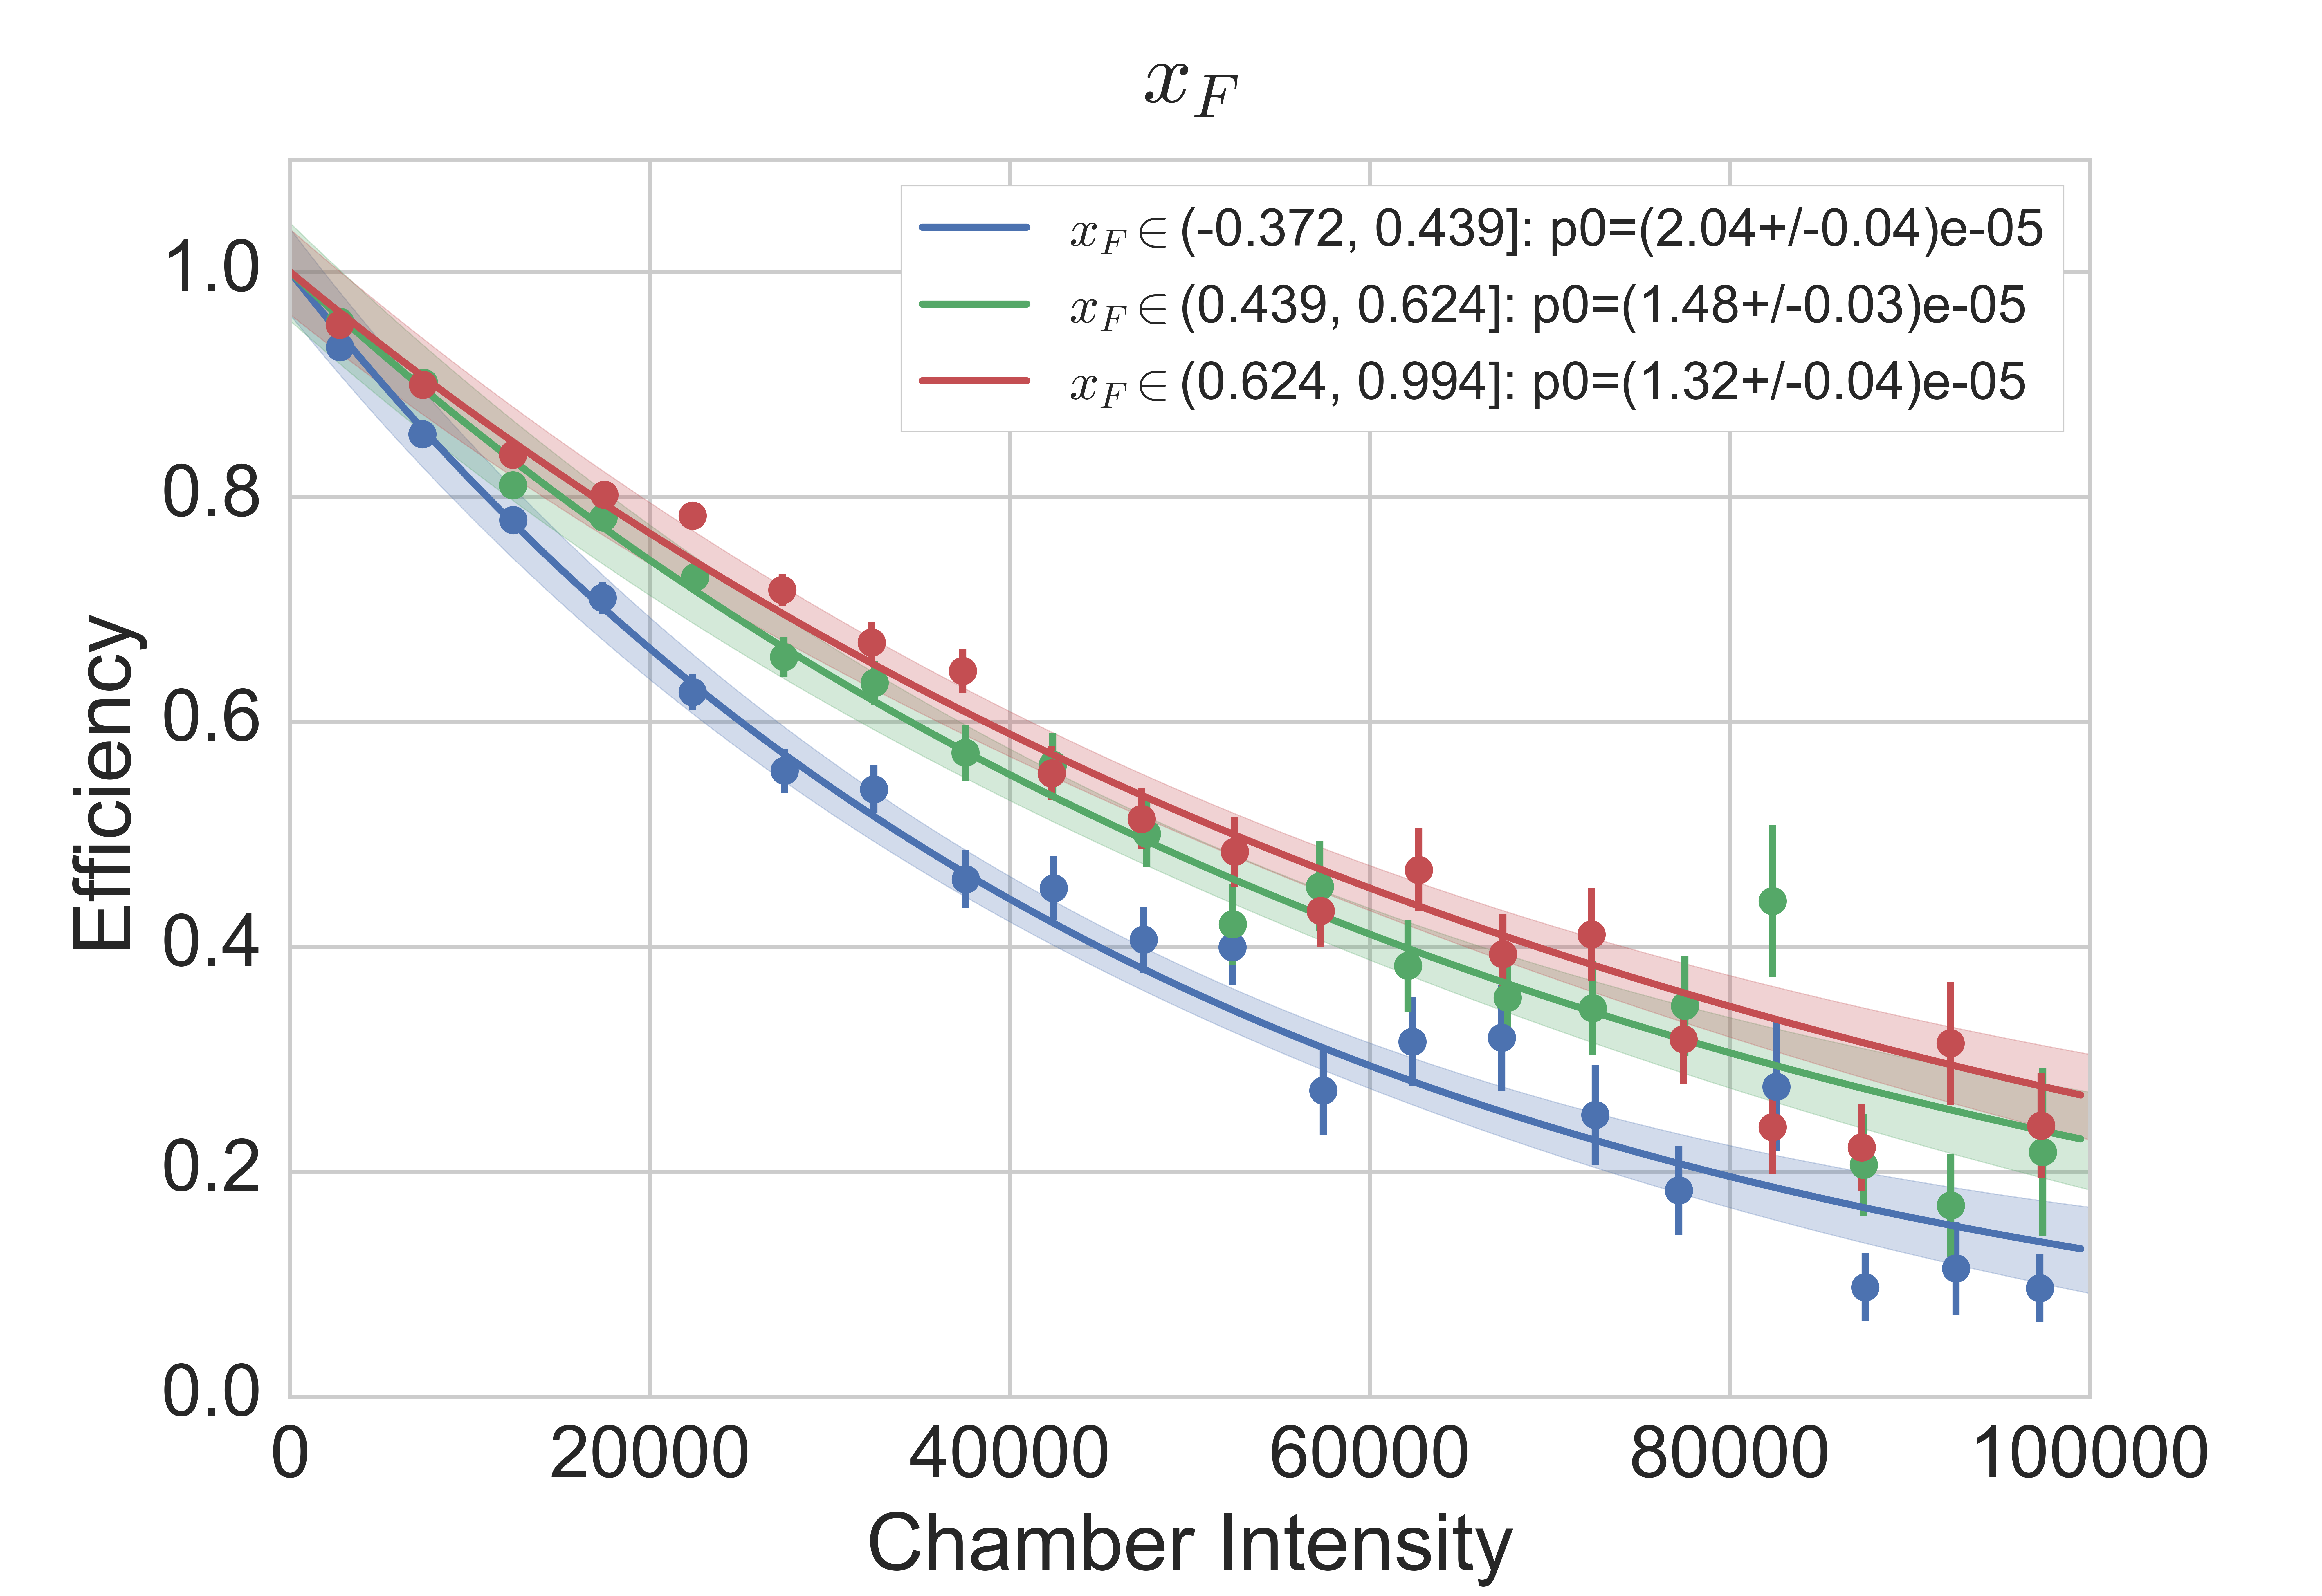
\includegraphics[width=0.49\textwidth]{figures/analysis/xF-keff-int.png}
	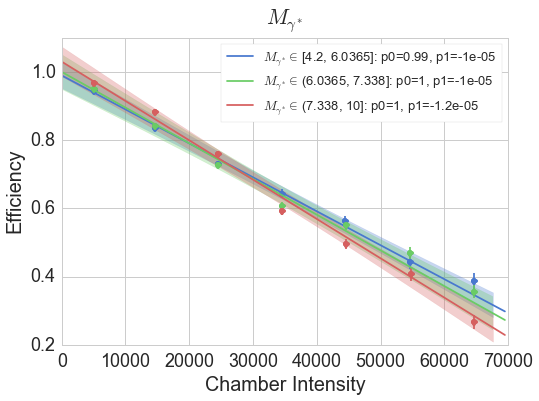
\includegraphics[width=0.49\textwidth]{figures/analysis/mass-keff-int.png}
	\caption{The kinematics $x_F$ and $M_{\gamma^*}$ are investigated. A clear kinematic dependence exists in $x_F$ while $M_{\gamma^*}$ is largely consistent.}
	\label{fig:keff-mass-xf}
\end{figure}

Another consideration is with respect to whether or not there is a target dependence to factor into the correction. For all of the above ``kEfficiency'' plots, only deuterium data is used. The kEfficiency curves for deuterium, hydrogen, carbon, iron, and tungsten can be found on Figure~\ref{fig:keff-target-roadset}. It can be concluded that there is enough of a difference between deuterium, iron, and the rest to justify calculating and applying this correction on a target-by-target basis.
\begin{figure}
	\centering
	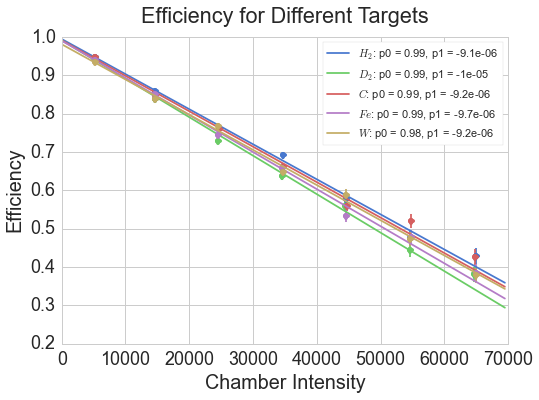
\includegraphics[width=0.49\textwidth]{figures/analysis/target-keff-int.png}
	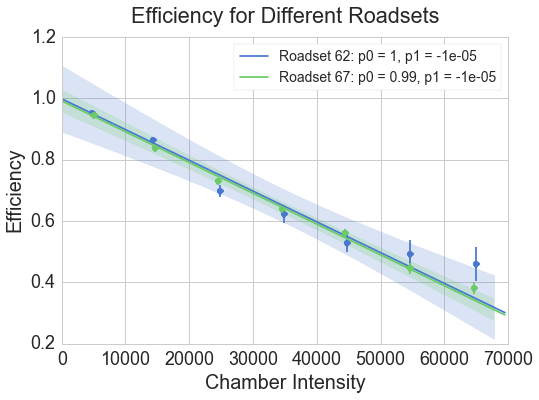
\includegraphics[width=0.49\textwidth]{figures/analysis/roadset-keff-int.png}
	\caption{Comparing the tracking efficiency curves across (left) the five targets and (right) two temporally different subsets (different roadsets) of data. Confidence bands removed from the target plot for the sake of clarity.}
	\label{fig:keff-target-roadset}
\end{figure}

Also, as a sanity check, there should be no time-dependence of this function. A quick check comparing different sets of data from two different roadsets quickly confirm that there is no such time dependence (Fig.~\ref{fig:keff-target-roadset}).

As a result, the final calculation of an tracking efficiency for a given dimuon event should depend on (1) target, (2) $x_F$, and (3) intensity. In order to apply this as a weight, we first define \emph{kEff}$_{t, \bar{x}}(I)$, a set of linear fit functions: one for each target (\emph{t}) and for each kinematic bin ($\bar{x}$), which may be binned in any number of kinematic dimensions. In the case of this analysis, the kinematic binning will only be in $x_F$. The procedure in weighting each dimuon will then be to take each dimuon event \emph{i} and its chamber intensity $I_i$, originating from target $t_i$ in $x_F$ bin $x_{F_i}$, create a weight as
\begin{equation}
w_i = \frac{1}{kEff_{t_i, x_{F_i}}(I_i)}
\end{equation}

\subsection{The Naive Empty/None Correction}

First a few values must be defined. An overall efficiency based on 'contributions' from the Empty/None background can be defined as

\begin{equation}
\epsilon_b = 1 - \frac{Y_b/p_b}{Y_t/p_t} = 1 - \left(\frac{p_t}{p_b}\right) \left( \frac{Y_b}{Y_t} \right)
\end{equation}

where Y is the dimuon \emph{yield} from a given target and \emph{p} is the integrated ``live proton'' count for the same given target. Here, $b \in \{Empty,\ None\}$ and $t\in\{H,\ D,\ C,\ Fe,\ W\}$. It is yet to be conclusively decided by the collaboration whether or not the Empty and None targets are to be combined for these calculations.

The next step is to adjust the yields with the \emph{kEff}$_{t,\bar{x}}(I)$:

\begin{equation}
Y_a \rightarrow Y_a^\prime = \sum_{i:i_t=a} \frac{1}{kEff_{t_i, x_i}(I_i)}
\end{equation}

The yield efficiency when factoring in background then becomes

\begin{equation}
\epsilon^\prime_b = 1 - \left(\frac{p_t}{p_b}\right) \left( \frac{Y^\prime_b}{Y^\prime_t} \right)
\end{equation}

\subsection{The Empty/None vs. Intensity Curve}


\subsection{Improved Background Correction}

With the Empty/None vs. Intensity Curve \emph{C(I)}, we can apply a more sophisticated correction. With C(I), we can make an expression for the background contribution to the yields of a given target:

\begin{equation}
p_t \left( \frac{Y^\prime_b}{p_b} \right) = \sum_{i:i_t=t} \frac{D\cdot C(I_i)}{kEff_{t_i, x_i}(I_i)}
\end{equation}
where D is a normalization constant defined in such a way that $D \cdot C(I)$ is the \% chance that a given dimuon from a target actually came from the Empty/None background. D can be calculated as
\begin{eqnarray}
D & = & \frac{1}{F} Y^\prime_b \left( \frac{p_t}{p_b} \right) \\
F & = &\sum_{i: i_t=t} \frac{C(I_i)}{kEff_{t_i, x_i}(I_i)}
\end{eqnarray}

The new intensity-dependent efficiency can now be defined as

\begin{equation}
(\epsilon_b^\prime)_i = 1 - D \cdot C(I_i)
\end{equation}

\section{Combinatorial Background Correction}

\red{Discuss analysis investigating results for the like-sign reconstruction to estimate the combinatorial background. Hopefully it will be intensity-dependent.}

\section{$ld_2$ Contamination Correction}

\red{Discuss contamination backstory, composition breakdown, the fluctuation from bottle-to-bottle, the correction procedure, and the proposed systematic uncertainty in that procedure.}

\section{Isoscalar Corrections for $^{183}W$ and $^{56}Fe$}

\red{Give brief correction in approximating n==p conversion. Be sure to show results for both iso-corrected and not!}

